\documentclass[letterpaper, reqno,11pt]{article}
\usepackage[margin=1.0in]{geometry}
\usepackage{color,latexsym,amsmath,amssymb,graphicx,float,listings,tikz,xcolor}
\usepackage{hyperref}

\hypersetup{
colorlinks=true,
linkcolor=magenta,
filecolor=magenta,
urlcolor=cyan,
}

\lstset{
basicstyle=\ttfamily,
columns=fullflexible,
frame=single,
breaklines=true,
postbreak=\mbox{\textcolor{red}{$\hookrightarrow$}\space},
}

\graphicspath{ {images/} }

\begin{document}

\begin{titlepage}
\newgeometry{margin=3cm}
\centering

\vspace*{\stretch{2}}

\Large Investigation of Fourier Optics in Fraunhofer and Fresnel Limits

\normalsize

\vspace{\stretch{1}}

% \normalsize Power Supplies and Voltage Regulators

\vspace{\stretch{0.5}}

\begin{tabular}{ll}
Name & Xander Naumenko \\[2ex]
Student number & 38198354 \\[2ex]
Partner & Renu Rajamagesh \\[2ex]
Lab name & Fourier optics \\[2ex]
Lab station  & L2C \\[2ex]
Assigned TA            & ? \\[2ex]
Lab \#            & 1 \\[2ex]
Notes &  N/A
\end{tabular}

\vspace{\stretch{3}}


\vspace{\stretch{2}}
\end{titlepage}

\begin{abstract}
    In the far field limit or when using a lens, several techniques from Fourier analysis can be applied to optics to give somewhat surprising results. Several experiments were undertaken in this report to investigate these effects. First, the threshold for where Fourier optics are applicable was tested by observing diffraction patterns of a slit in various configuration. Next, a lens was used to observe the fourier transform of a mesh, text and a razor blade. This was used to optically recognize characters in the object plane, with no active computing required.
\end{abstract}

\newpage

\section{Research Note}

\subsection{Introduction}

One result from this report that is of significant interest is the filtering of low frequency light to enhance fine details. This technique can be used to optically enhance very fine detail in an imaging plane, with no active processing required. It does this by the use of Fourier optics.

\subsection{Methods}

A collimated beam is shined onto a razorblade with a piece of clear glass glued to it. It is then fed into a Fourier transform lens (FTL), and for ease of viewing a Fourier plane imaging lens (FPIL) is used image the result onto a further plane. A Rasberry Pi camera is controlled to take pictures of the laser after this. As the glass is transparent, if viewed regularly it's very difficult to make out the contour.

To increase this contrast, a small dot embedded in transparent acrylic is placed in the Fourier plane. With this insertion, the new image is recorded and be compared to the original.

\subsection{Theory}

At the focal distance after a lens, the light pattern inputted to the lens will have undergone a Fourier transform. By using a dot to filter all the spatial frequencies lower than a threshold, only the higher frequencies remain. Since contours and fine detail require high frequency to describe accurately, this leaves only them in the resulting image.

\subsection{Results}

The resulting image has a contour that is significantly attenuated, as can be seen in figure \ref{fig:rn}. This is very significant, since it makes the faint edges extremely visible. This has potential practical usage, as for a given object being imaged in a given experiment, this technique can be used to filter for the parts of the image that are composed of fine detail while ignoring any lower spatial frequency components that may be overcrowding the important signal.

\begin{figure}[h!]
    \centering
    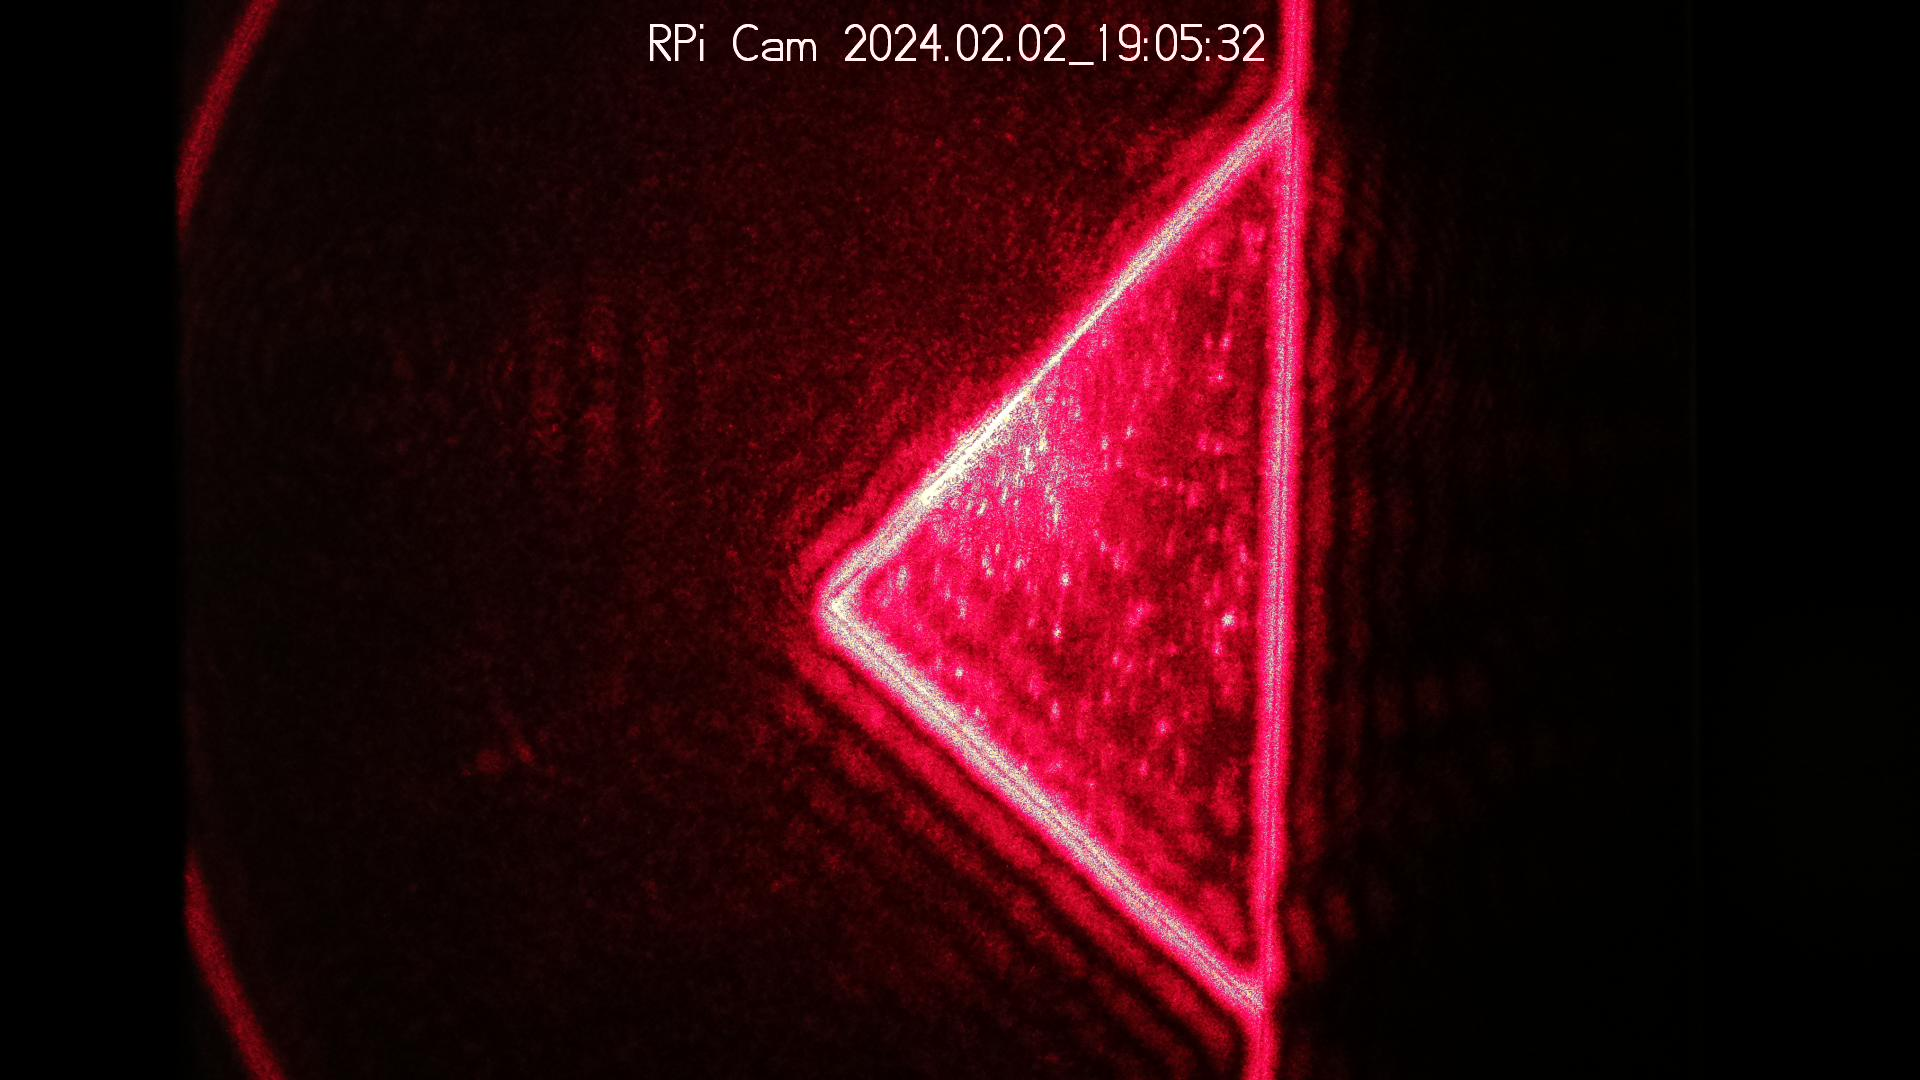
\includegraphics[width=0.7\textwidth]{Fourier/5g/media/im_0229_20240202_190532.jpg}
    \caption{The piece of glass (triangle) attached to the razorblade (right) after being filtered for low frequency light. Note how the edges are extremely attenuated.}
    \label{fig:rn}
\end{figure}

\newpage

\section{Experiments}


\textcolor{red}{\noindent 2.3.1A.} The alignment was fairly straightforward in our case, as the previous team had already left it in a state close to aligned. As suggested in the instructions, we made small adjustments using a blank sheet of paper to measure the degree of existing misalignment. See figure \ref{fig:2-3-1A} for an example of this process.

\begin{figure}[tb]
    \centering
    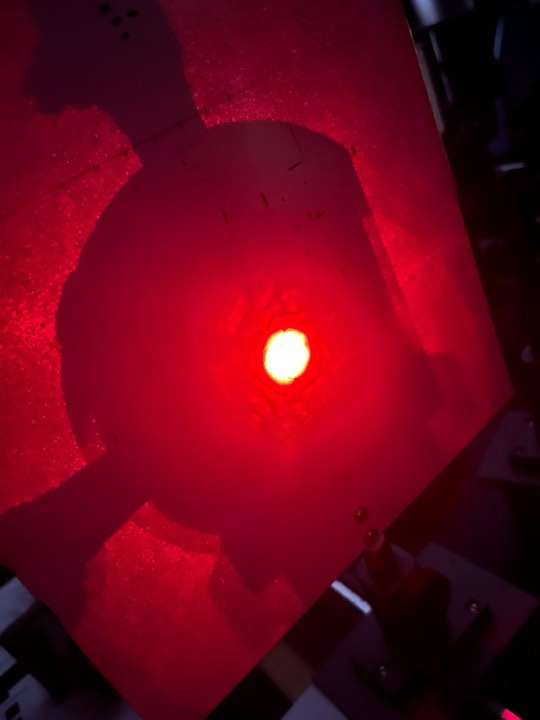
\includegraphics[width=0.3\textwidth]{2.3.1A}
    \caption{Picture of setting up for 2.3.1A, a reference white background far away from the source was used to determine whether the laser was aligned.}
    \label{fig:2-3-1A}
\end{figure}

\noindent \textcolor{red}{2.3.2A.} See figure \ref{fig:2-3-2A} for the calibration picture. Using GIMP, the measured mm/pixel was found to be $0.0658$mm/pixel.

\begin{figure}[tb]
    \centering
    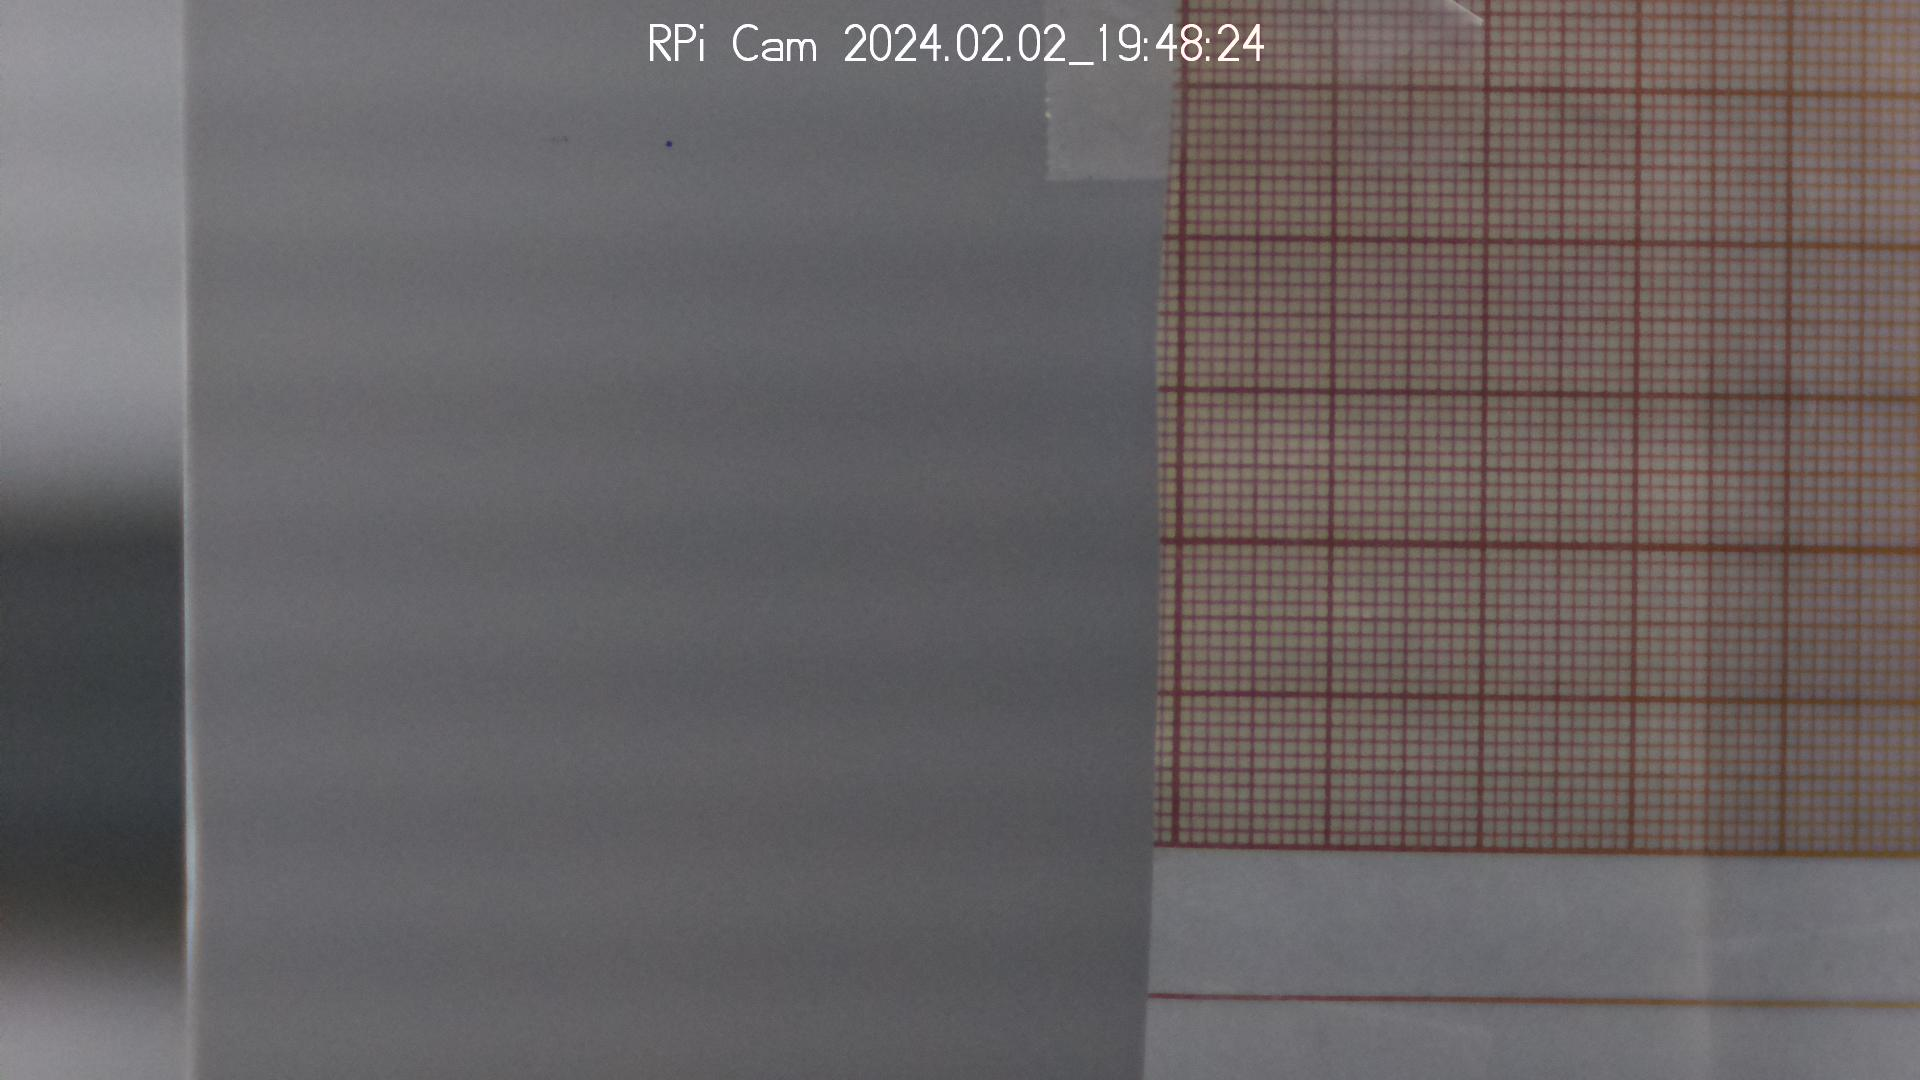
\includegraphics[width=0.5\textwidth]{Fourier/scale.jpeg}
    \caption{Scale used for all images in 2.3.2. This can be used to convert between pixels and millimeters.}
    \label{fig:2-3-2A}
\end{figure}

\noindent \textcolor{red}{2.3.2B.} From the definition of the Fraunhofer limit, that regime starts at $\frac{x^2}{\lambda}=\frac{z}{\pi}$. Note that in generally Fraunhofer is for $\frac{w^2}{\lambda}\ll\frac{z}{\pi}$, but given the open endedness of the question I'll use equality here and investigate when it's smaller in the next question. In this case, this gives a value of $w= \sqrt{ \frac{z\lambda}{\pi}}=0.88$mm. See figure \ref{fig:2-3-2B} for the resulting diffraction pattern. It is what we'd expect. The fringes that we expect in the far field limit are faint but beginning to be visible. The reason we expect the fringes in the Fraunhofer limit is that the slit is effectively a rect function, and the fourier transform of a rect function is sinc which has periodic decaying fringes.

\begin{figure}[tb]
    \centering
    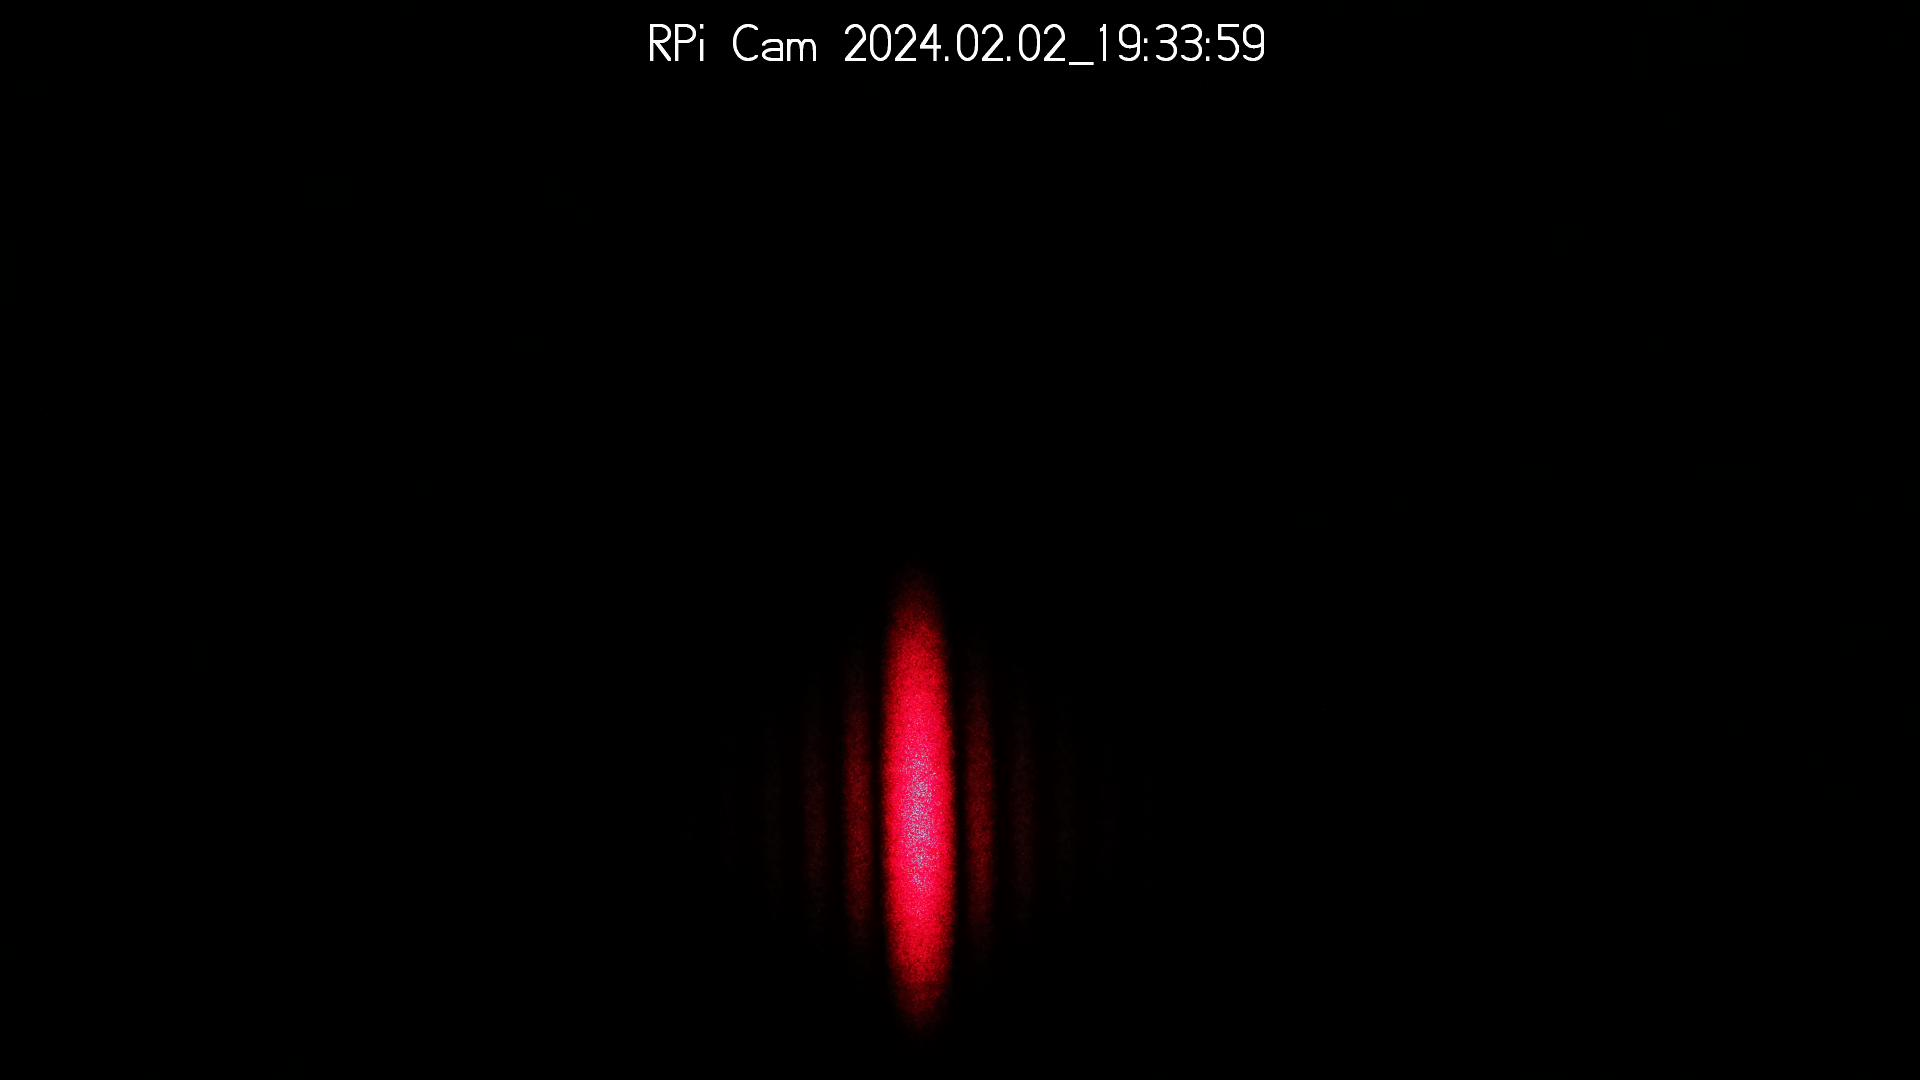
\includegraphics[width=0.7\textwidth]{Fourier/1_redo/media/im_0253_20240202_193359.jpg}
    \caption{Diffraction pattern for 2.3.2B of a single slit at beginning of the Fraunhofer limit, the fringes are somewhat visible but faint as expected.}
    \label{fig:2-3-2B}
\end{figure}

\noindent \textcolor{red}{2.3.2C.} See figure \ref{fig:3-2-2C}, as the question suggests the fringes get more intense and closer together during the transition between Fraunhofer and Fresnel.

\begin{figure}[tb]
    \centering
    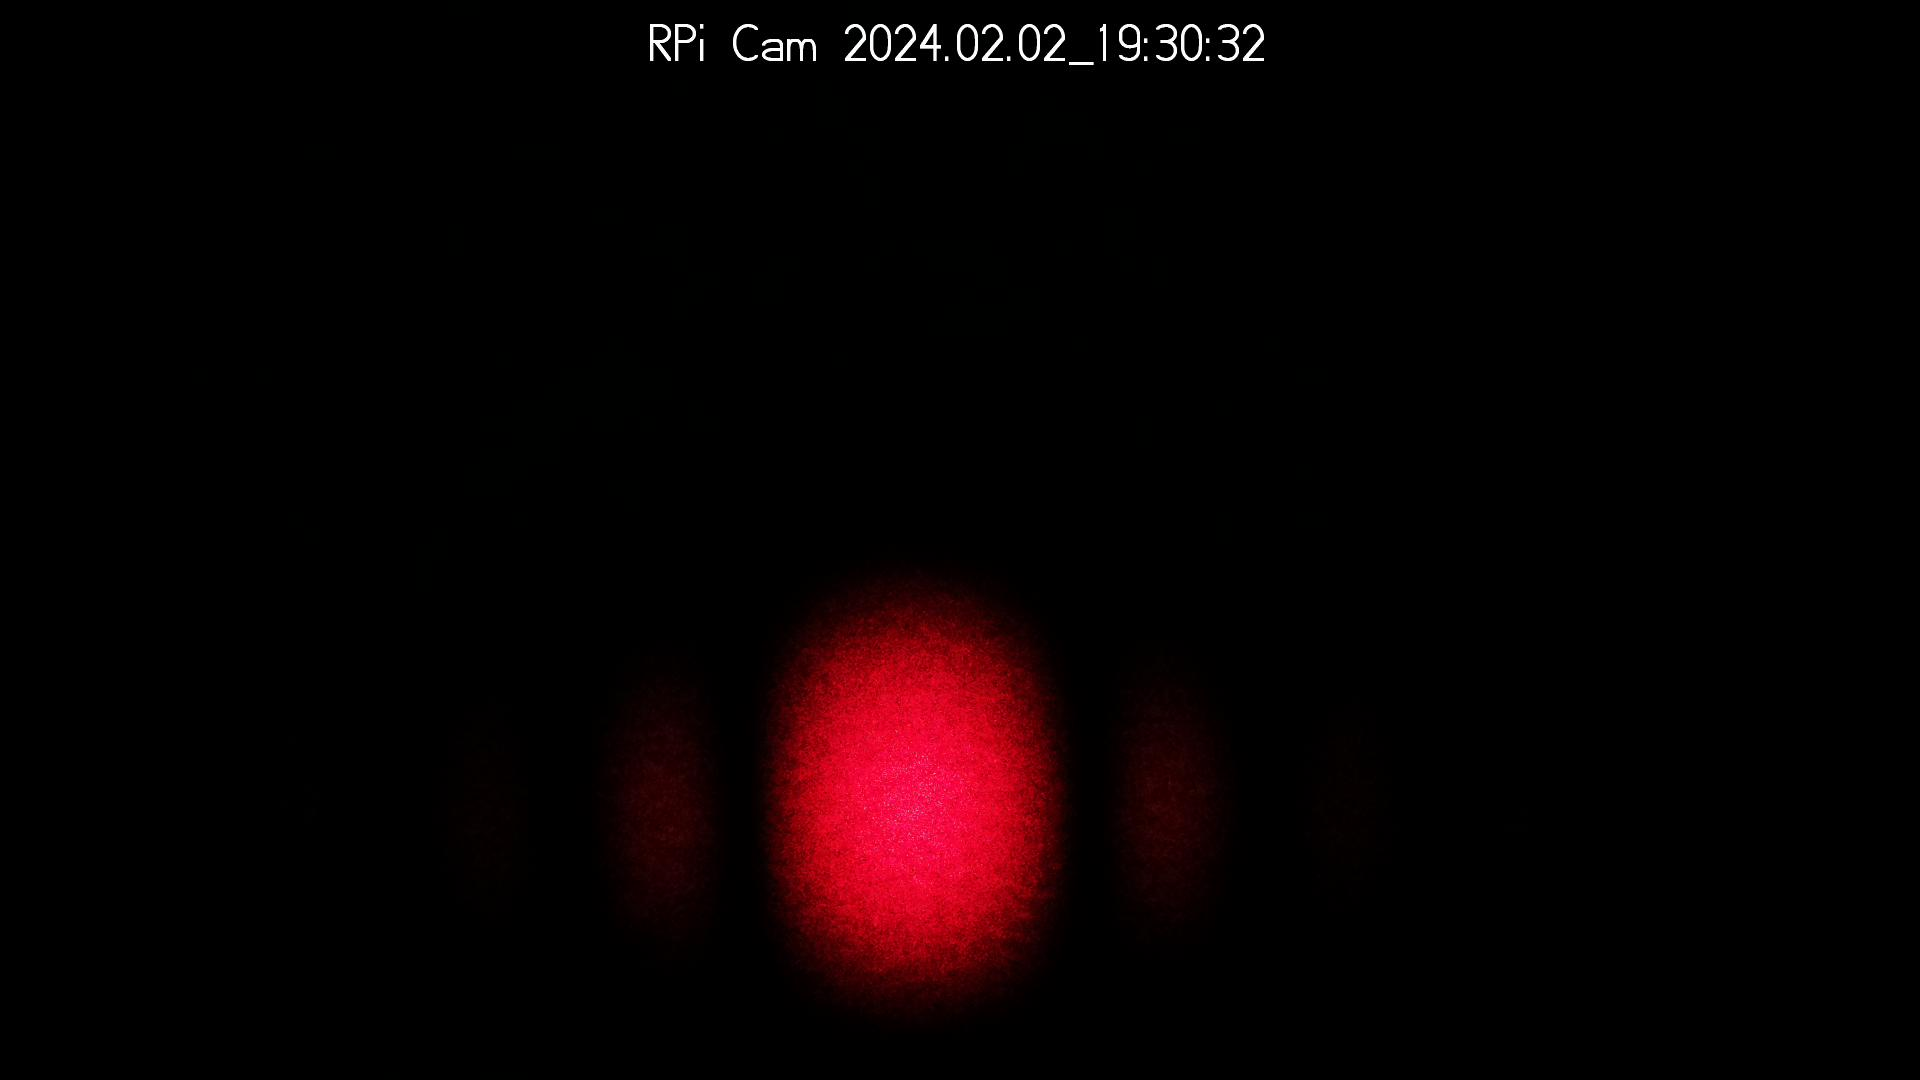
\includegraphics[width=0.45\textwidth]{Fourier/0.25_redo/media/im_0248_20240202_193032.jpg}
    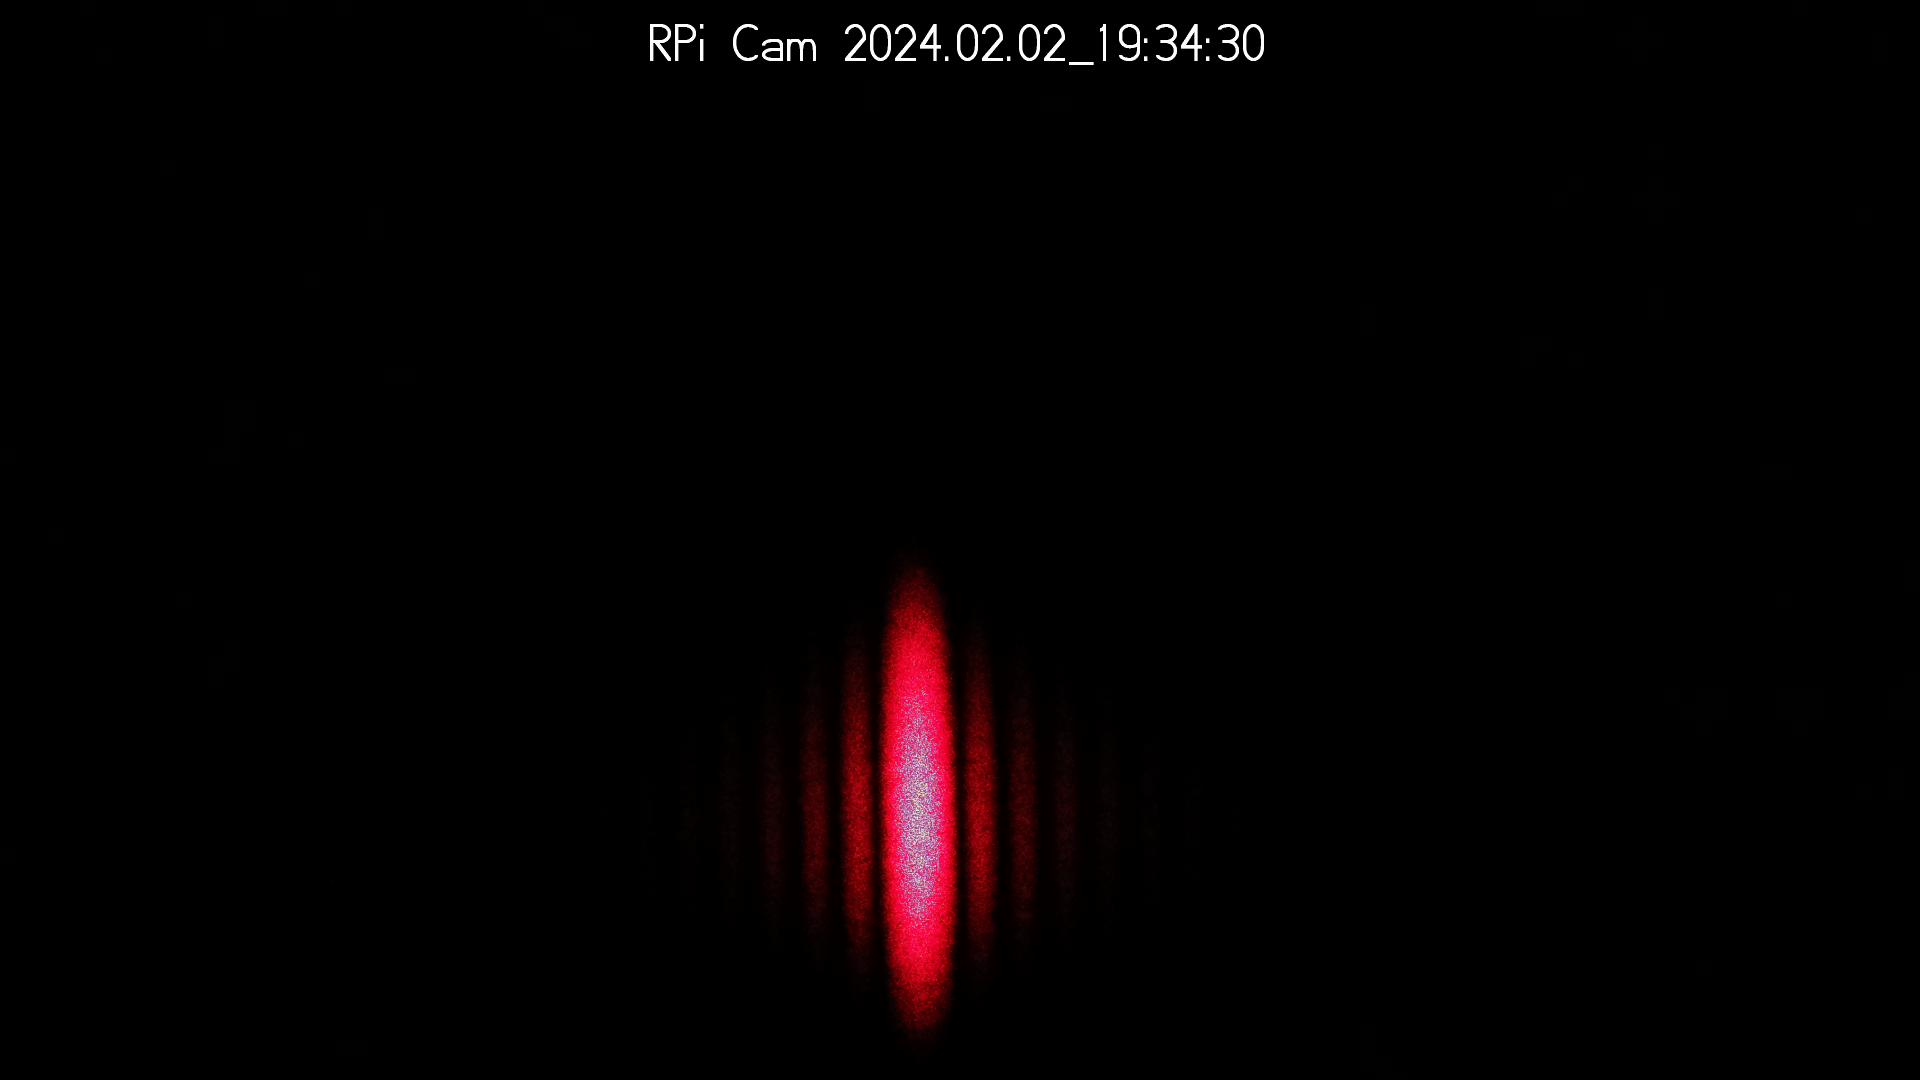
\includegraphics[width=0.45\textwidth]{Fourier/1_redo/media/im_0254_20240202_193430.jpg}
    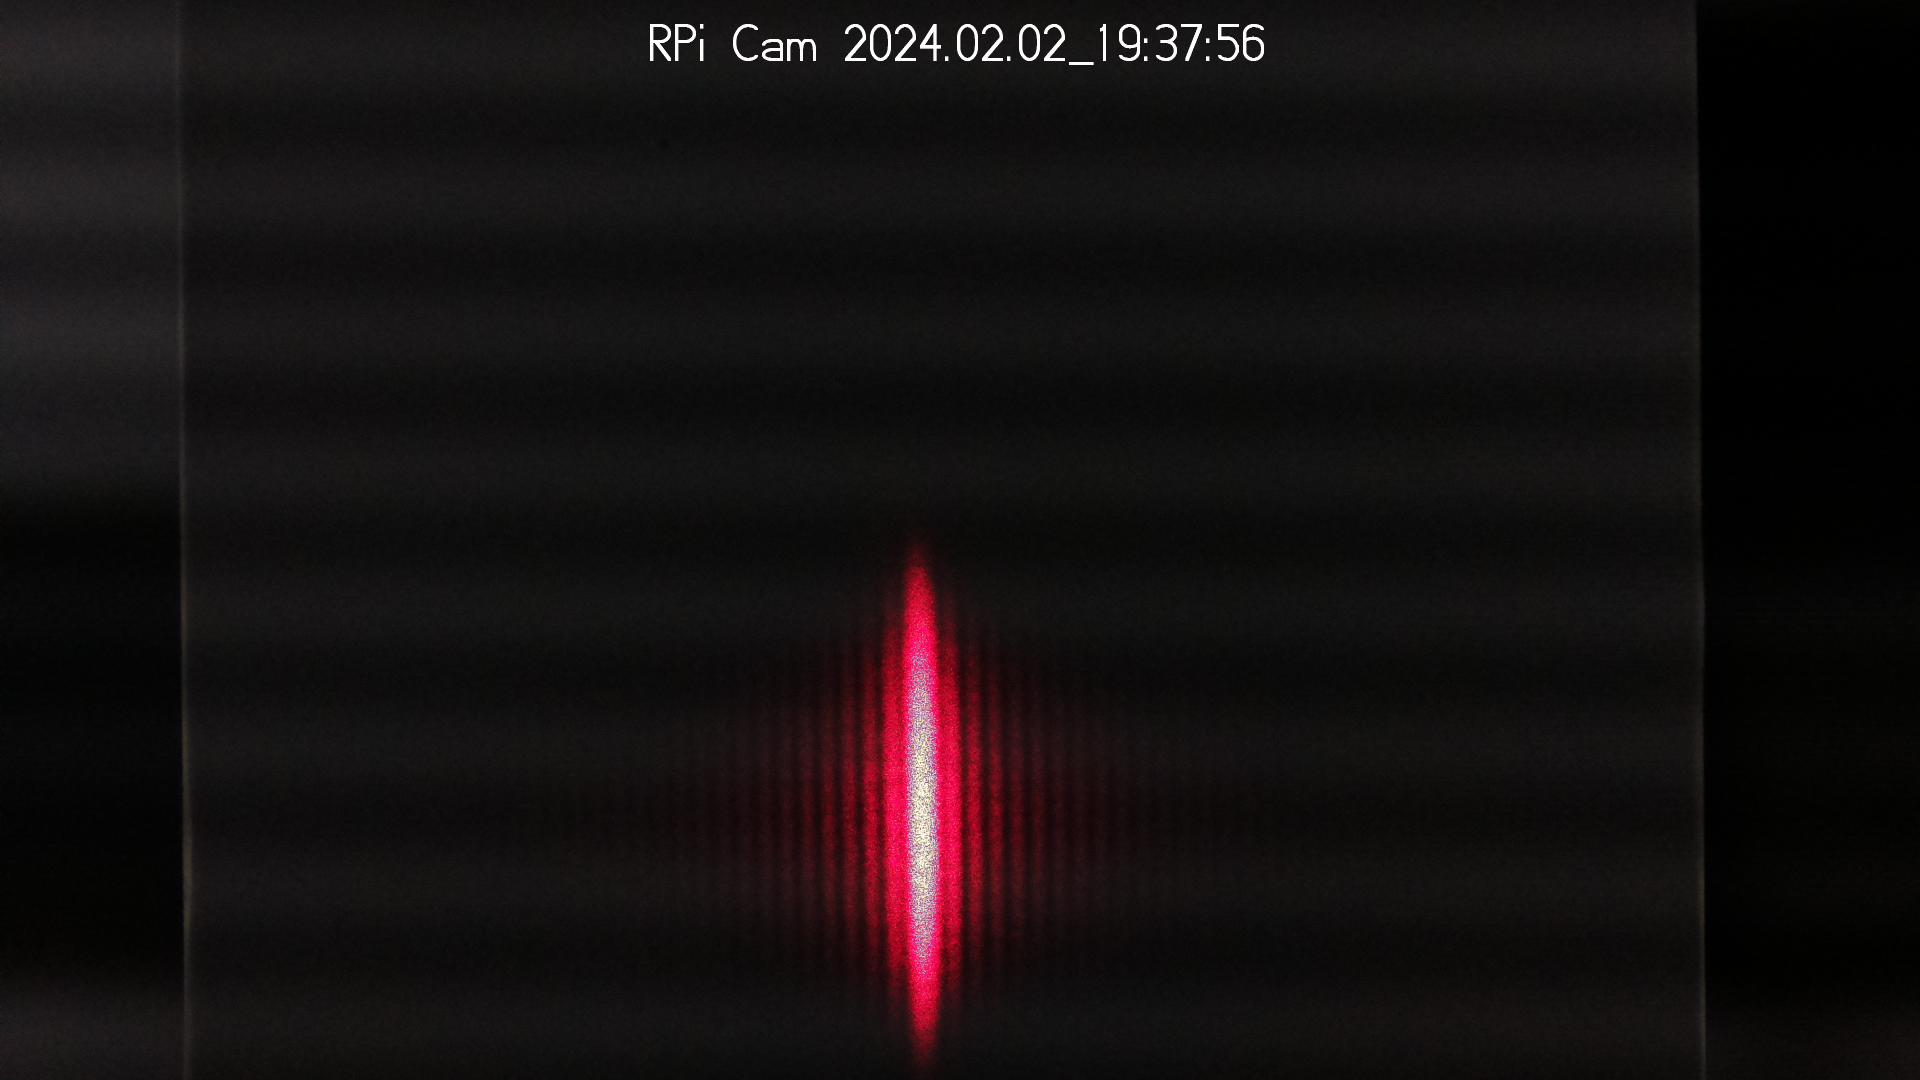
\includegraphics[width=0.45\textwidth]{Fourier/2_redo/media/im_0258_20240202_193756.jpg}
    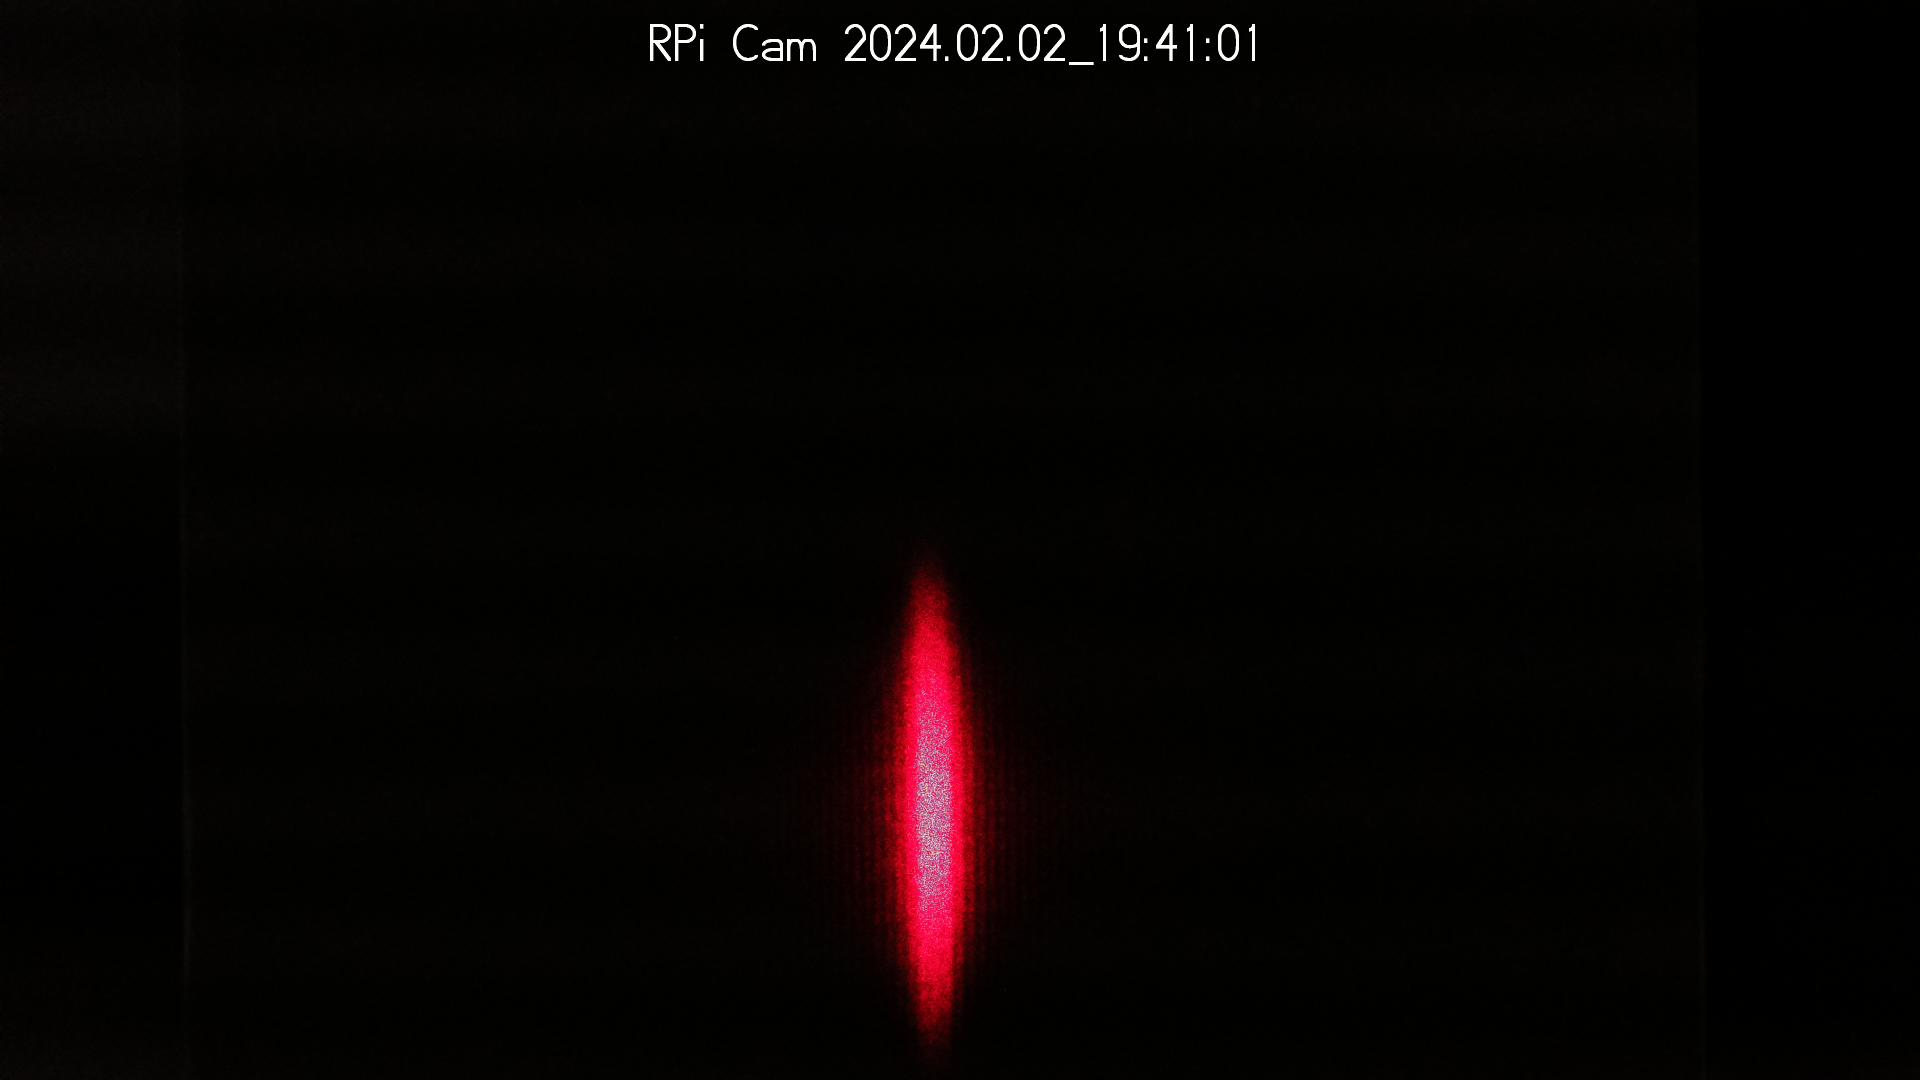
\includegraphics[width=0.45\textwidth]{Fourier/4_redo/media/im_0265_20240202_194101.jpg}
    \caption{Crossover from Fresnel to Fraunhofer limit of a slit. From top left to bottom right is increasing the width of the slit from $w /\sqrt{\lambda z /\pi}=0.25$ to $4$, the decreased spacing of the fringes clearly shows the transition between the two regimes.}
    \label{fig:3-2-2C}
\end{figure}

\noindent \textcolor{red}{2.3.2D.} See figure \ref{fig:3-2-2D}. Here is the code used:
\begin{lstlisting}
from PIL import Image
import numpy as np
import matplotlib.pyplot as plt

cx = 920
cy = 800
w = 400
h = 200
crop_area = (cx-w, cy-h, cx+w, cy+h)

files = [
    'Fourier/0.25_redo/media/im_0248_20240202_193032.jpg',
    'Fourier/1_redo/media/im_0254_20240202_193430.jpg',
    'Fourier/2_redo/media/im_0258_20240202_193756.jpg',
    'Fourier/4_redo/media/im_0265_20240202_194101.jpg',
]

imgs = [np.array(Image.open(file).convert('L').crop(crop_area)) for file in files]

I = [im.sum(axis=0) for im in imgs]

px_to_mm = 0.0658
dists = [0.25, 1, 2, 4]

X = np.linspace(-w*px_to_mm, w*px_to_mm, 2*w)

fig, axs = plt.subplots(4, 1, figsize=(10, 8), sharex=True, sharey=True)
fig.suptitle('Cross Section Intensity of Slit Diffraction')

for i, intensity in enumerate(I):
    axs[i].plot(X, intensity)
    axs[i].set_title("Intensity for $w /\\sqrt{\\lambda z/\\pi}=$ "+str(dists[i]))

for ax in axs:
    ax.set_xlabel('Position (mm)')
    ax.set_ylabel('Intensity (Arbitrary Scale)')

plt.tight_layout(rect=[0, 0.03, 1, 0.95])
plt.show()

\end{lstlisting}

\begin{figure}[tb]
    \centering
    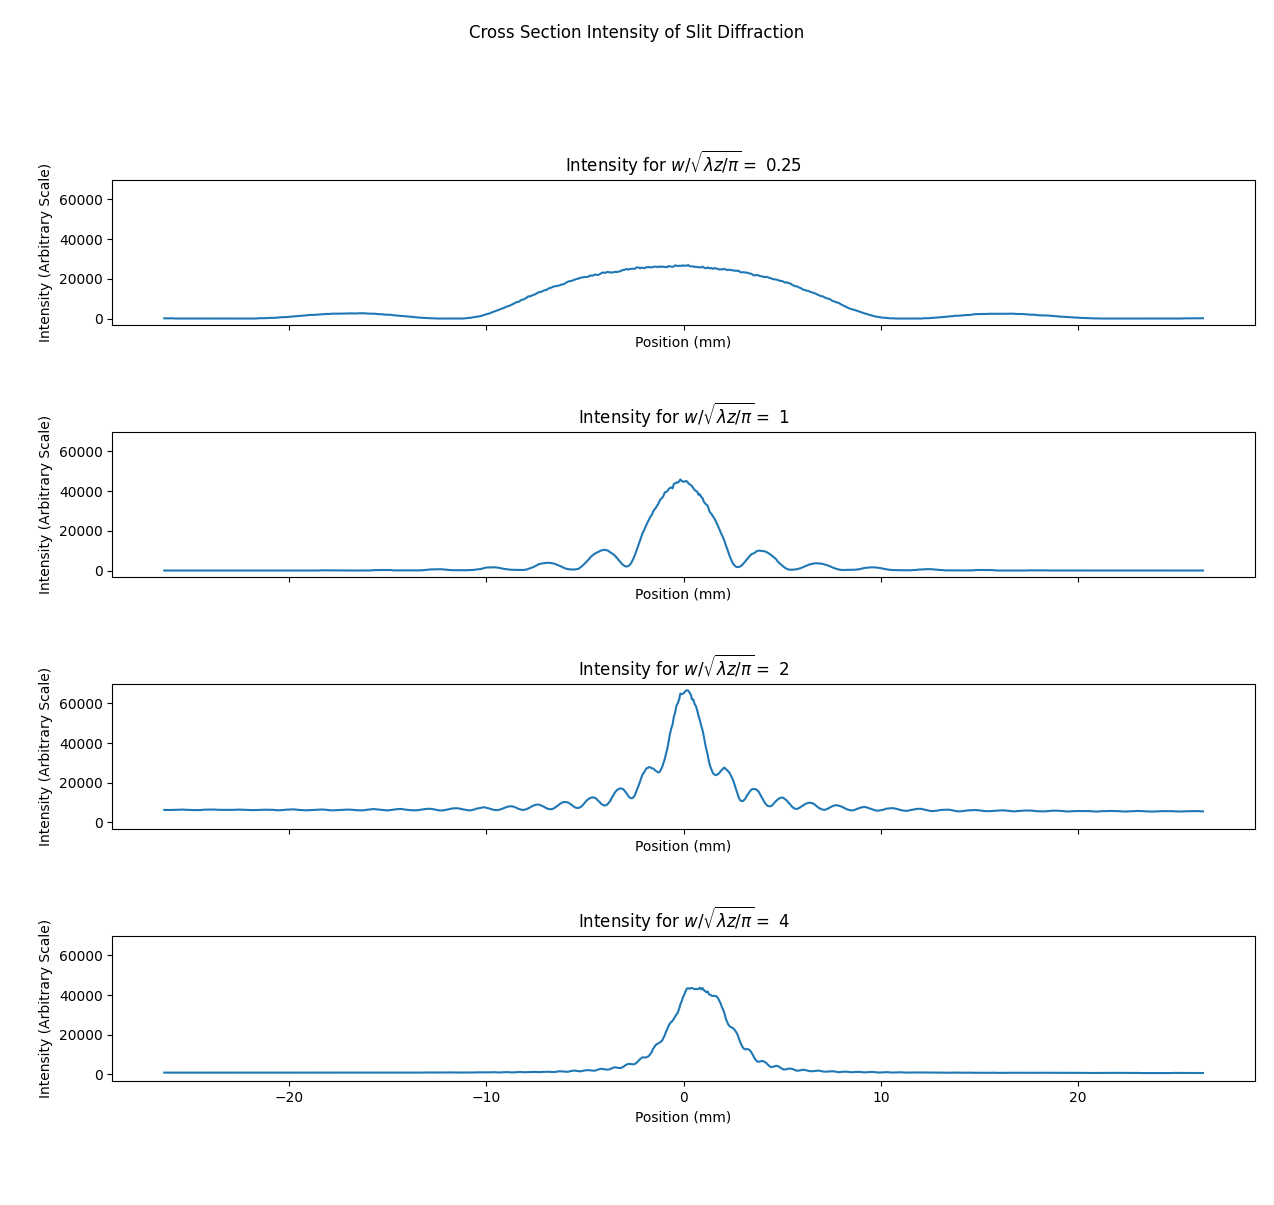
\includegraphics[width=0.8\textwidth]{3-2-2D}
    \caption{Intensity plots for question 3.2.2D. As expected, the transition between Fresnel and Fraunhofer regimes is clear.}
    \label{fig:3-2-2D}
\end{figure}
 
\noindent \textcolor{red}{2.3.3A.} See figure \ref{fig:2-3-3A}. The NOZONE negative is much more convenient than the other objects like the mesh, since it's very clear when it comes in focus. The letters become blurry if it's not exactly at the object plane, whereas for a mesh the dots just get a bit bigger and it's hard to tell the difference.

\begin{figure}[tb]
    \centering
    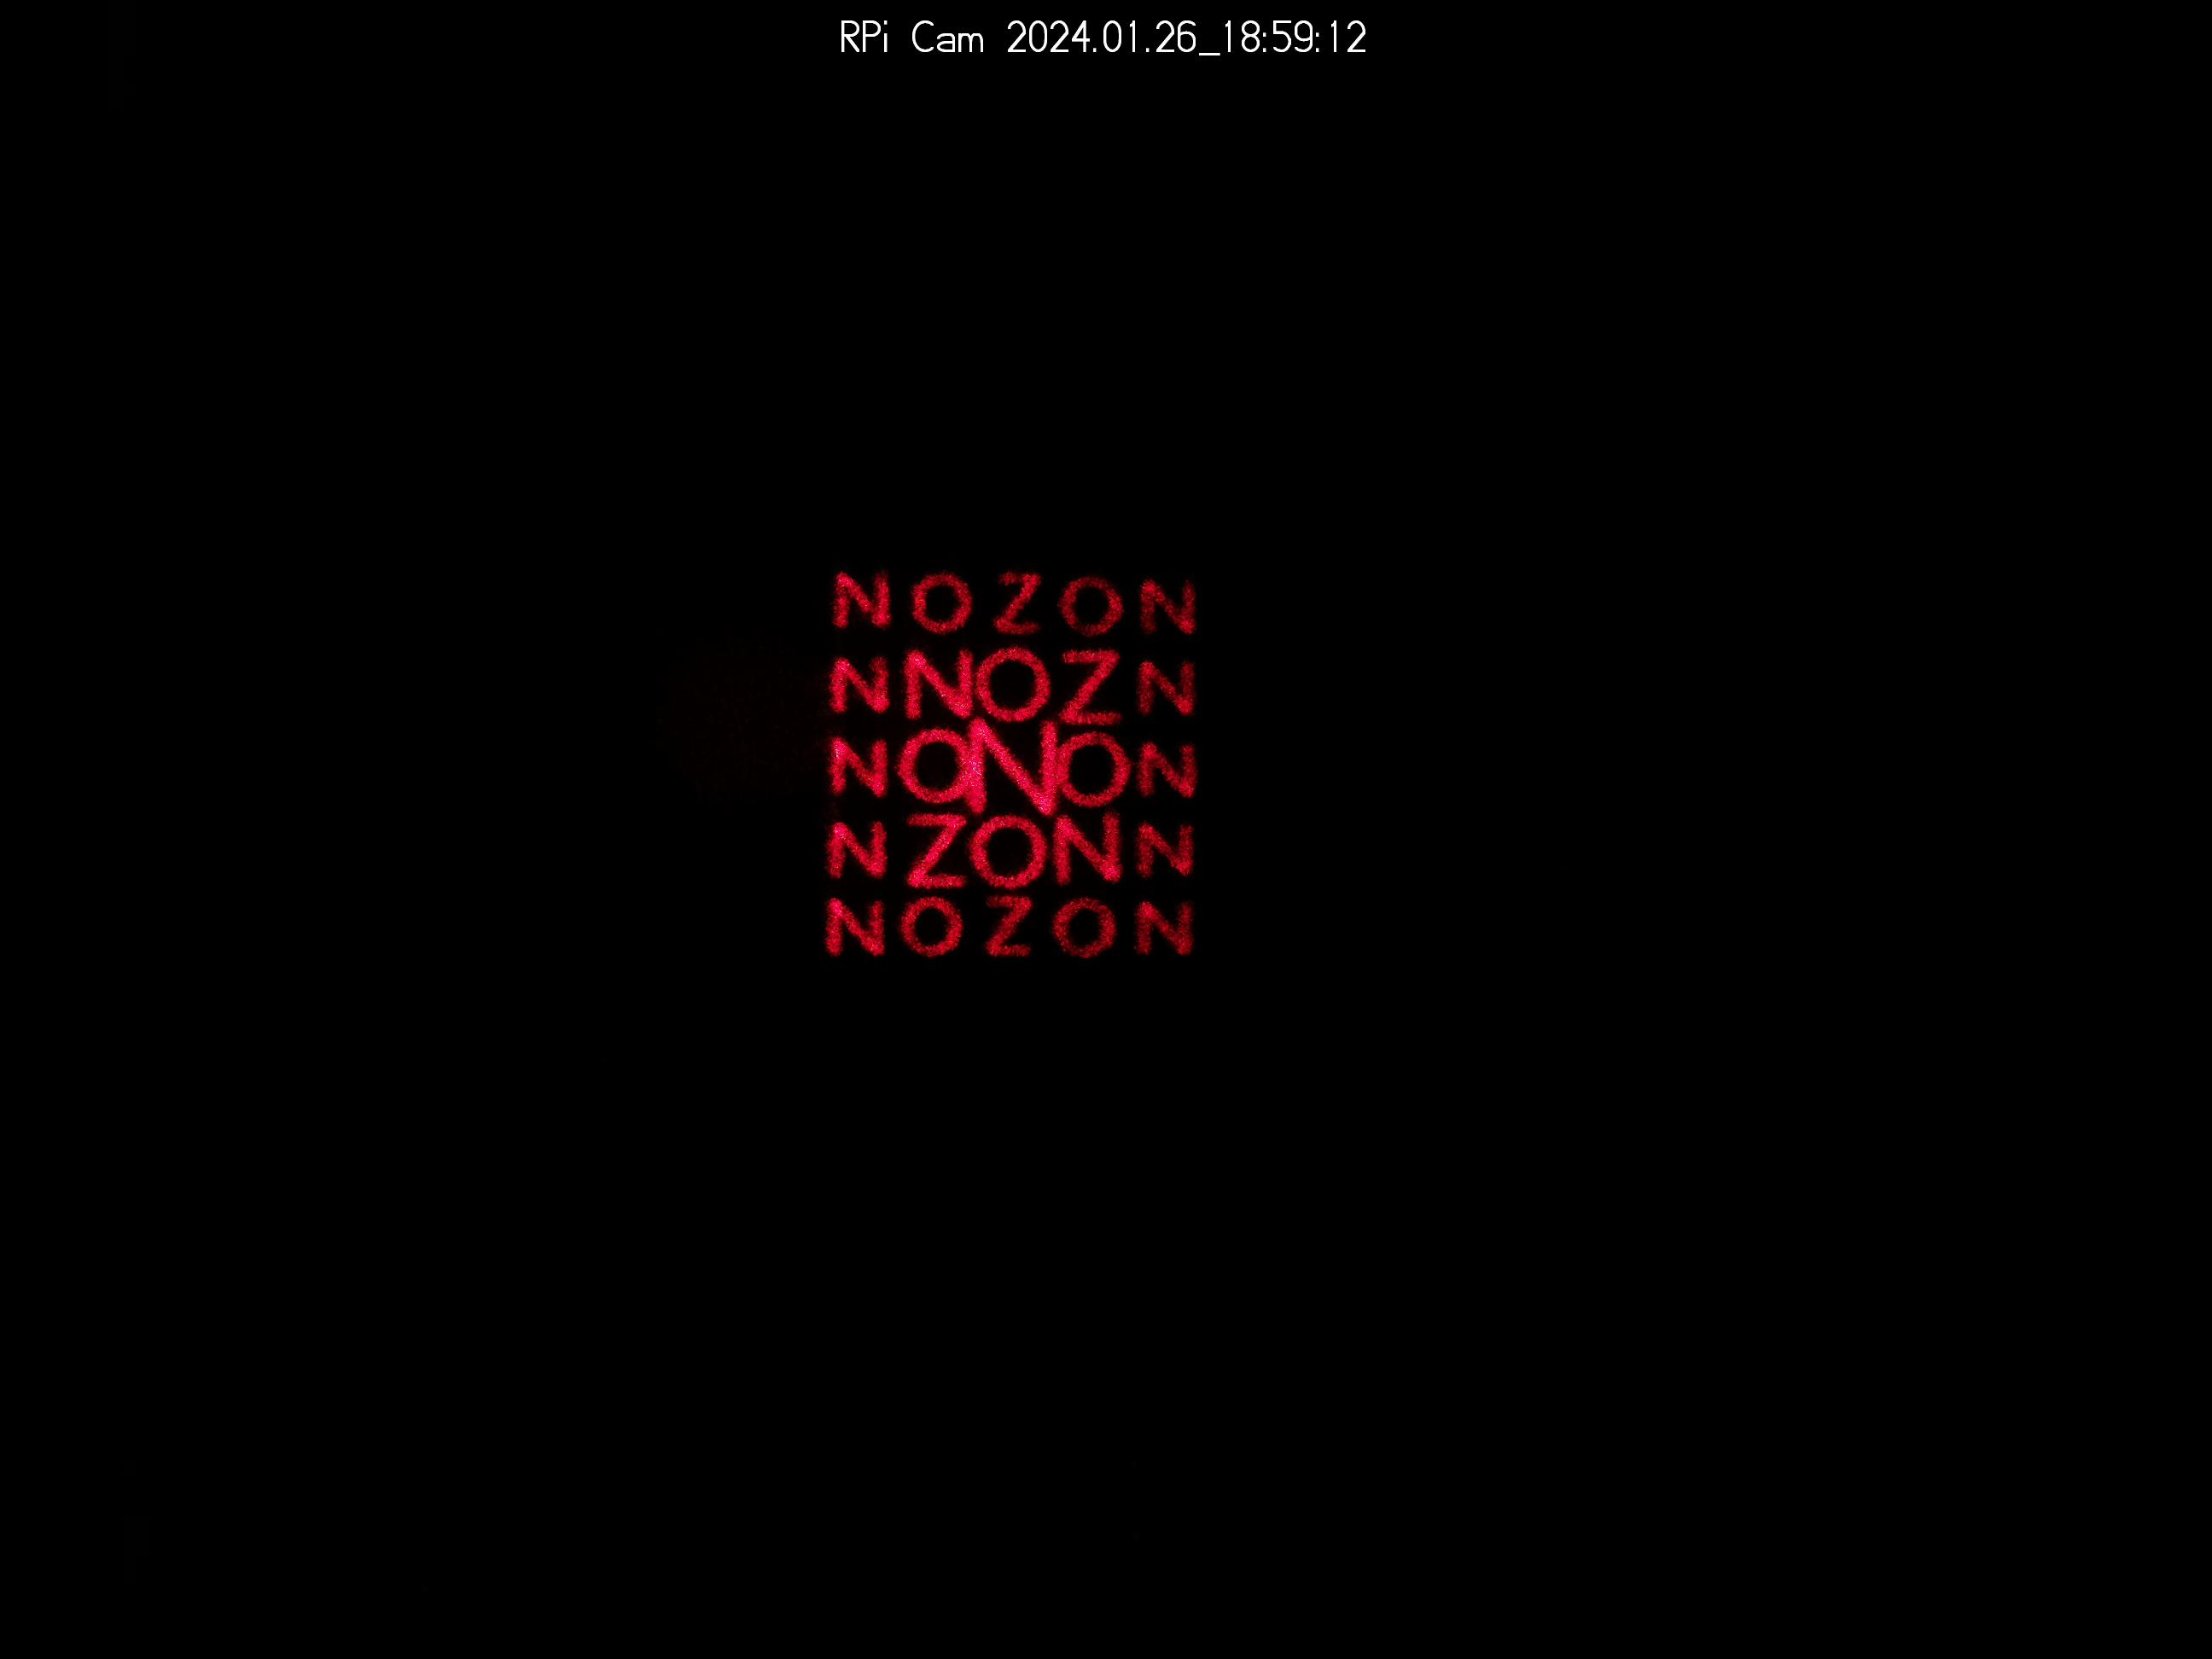
\includegraphics[width=0.5\textwidth]{Fourier/2A/media/im_0071_20240126_185912.jpg}
    \caption{NOZONE being used to find the object plane.}
    \label{fig:2-3-2A}
\end{figure}

\noindent \textcolor{red}{2.3.3B.} See figure \ref{fig:2-3-3B}. We have the wire spacing of 40 gaps/cm, and by measuring the image there are 29.25 pixels between each point. This gives
\[
\text{Magnification Ratio} = \frac{x'}{x}=\frac{29.25\cdot 0.05}{0.25}=5.85
.\]

\begin{figure}[tb]
    \centering
    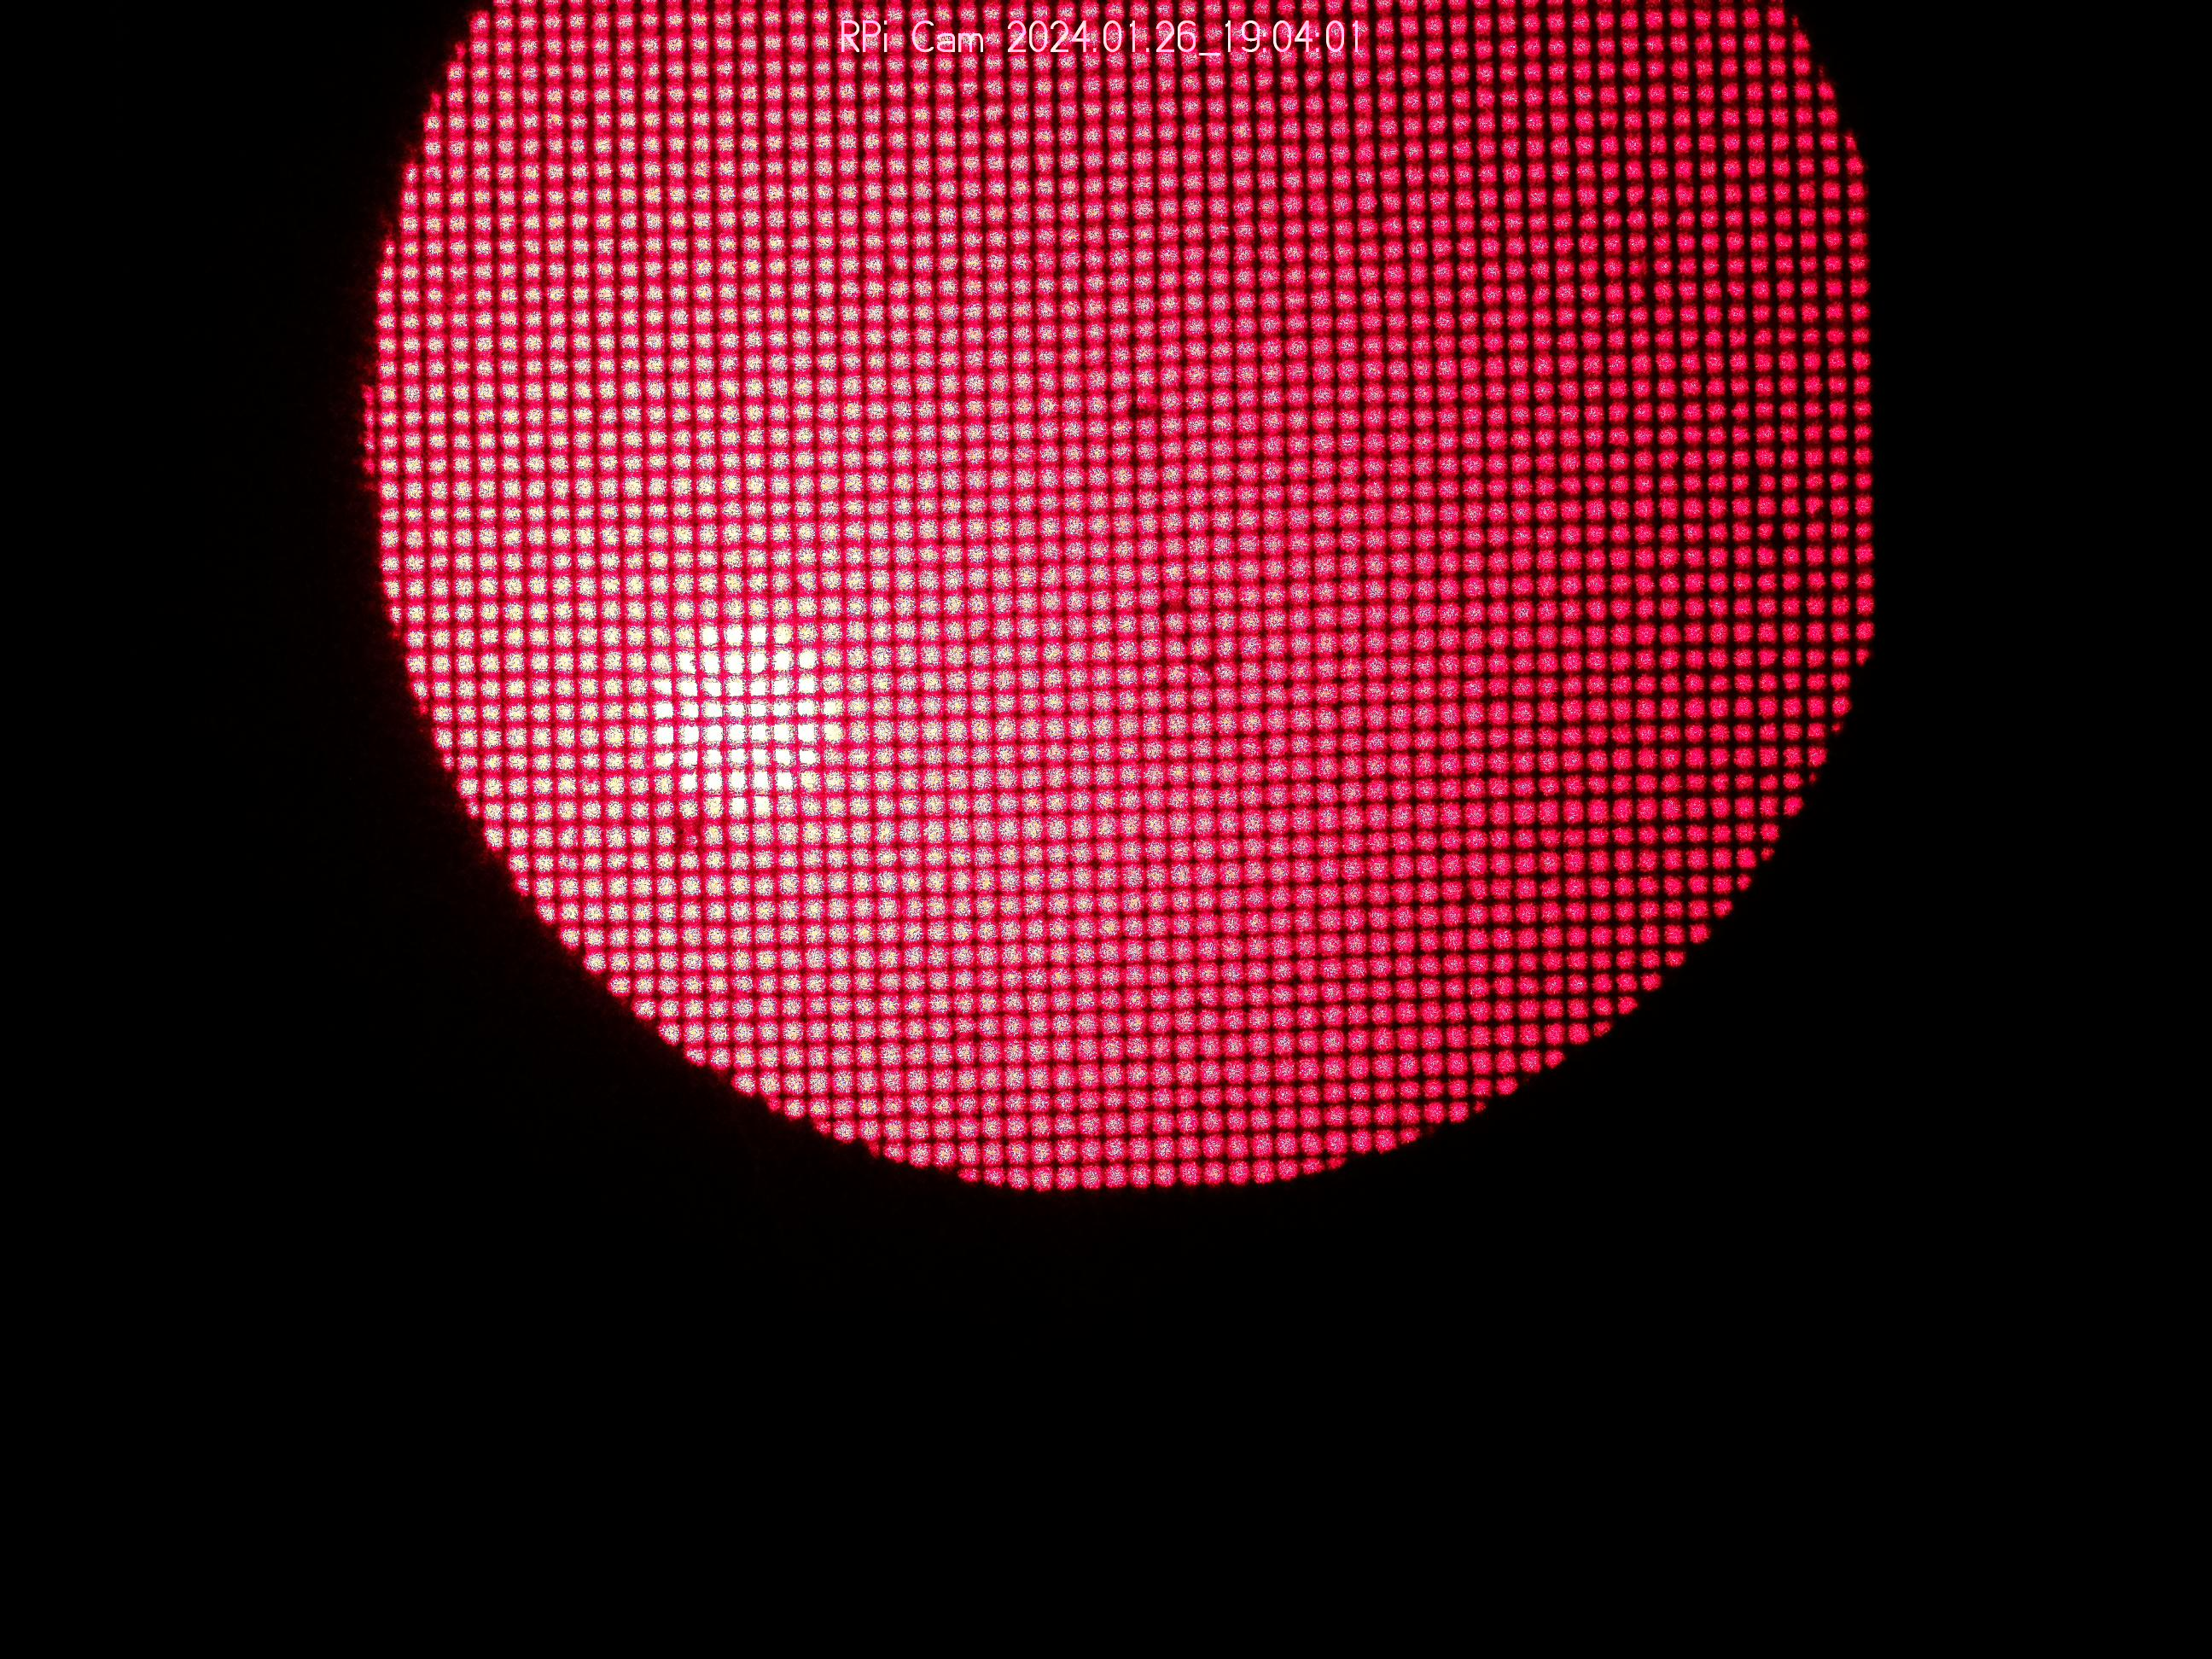
\includegraphics[width=0.5\textwidth]{Fourier/2B/media/im_0076_20240126_190401.jpg}
    \caption{Mesh in the object plane, used to find the magnification ratio.}
    \label{fig:2-3-3B}
\end{figure}

\noindent \textcolor{red}{2.3.3C.} We followed the procedure and found the Fourier plane at approximately 37cm from the Fourier transform lens. This is around where we'd expect, although we didn't have strong priors on where it should be given it should be at the somewhat arbitrary focal point of the lens. See figure \ref{fig:2-3-3C} for the resulting Fourier transform of the mesh.

\begin{figure}[tb]
    \centering
    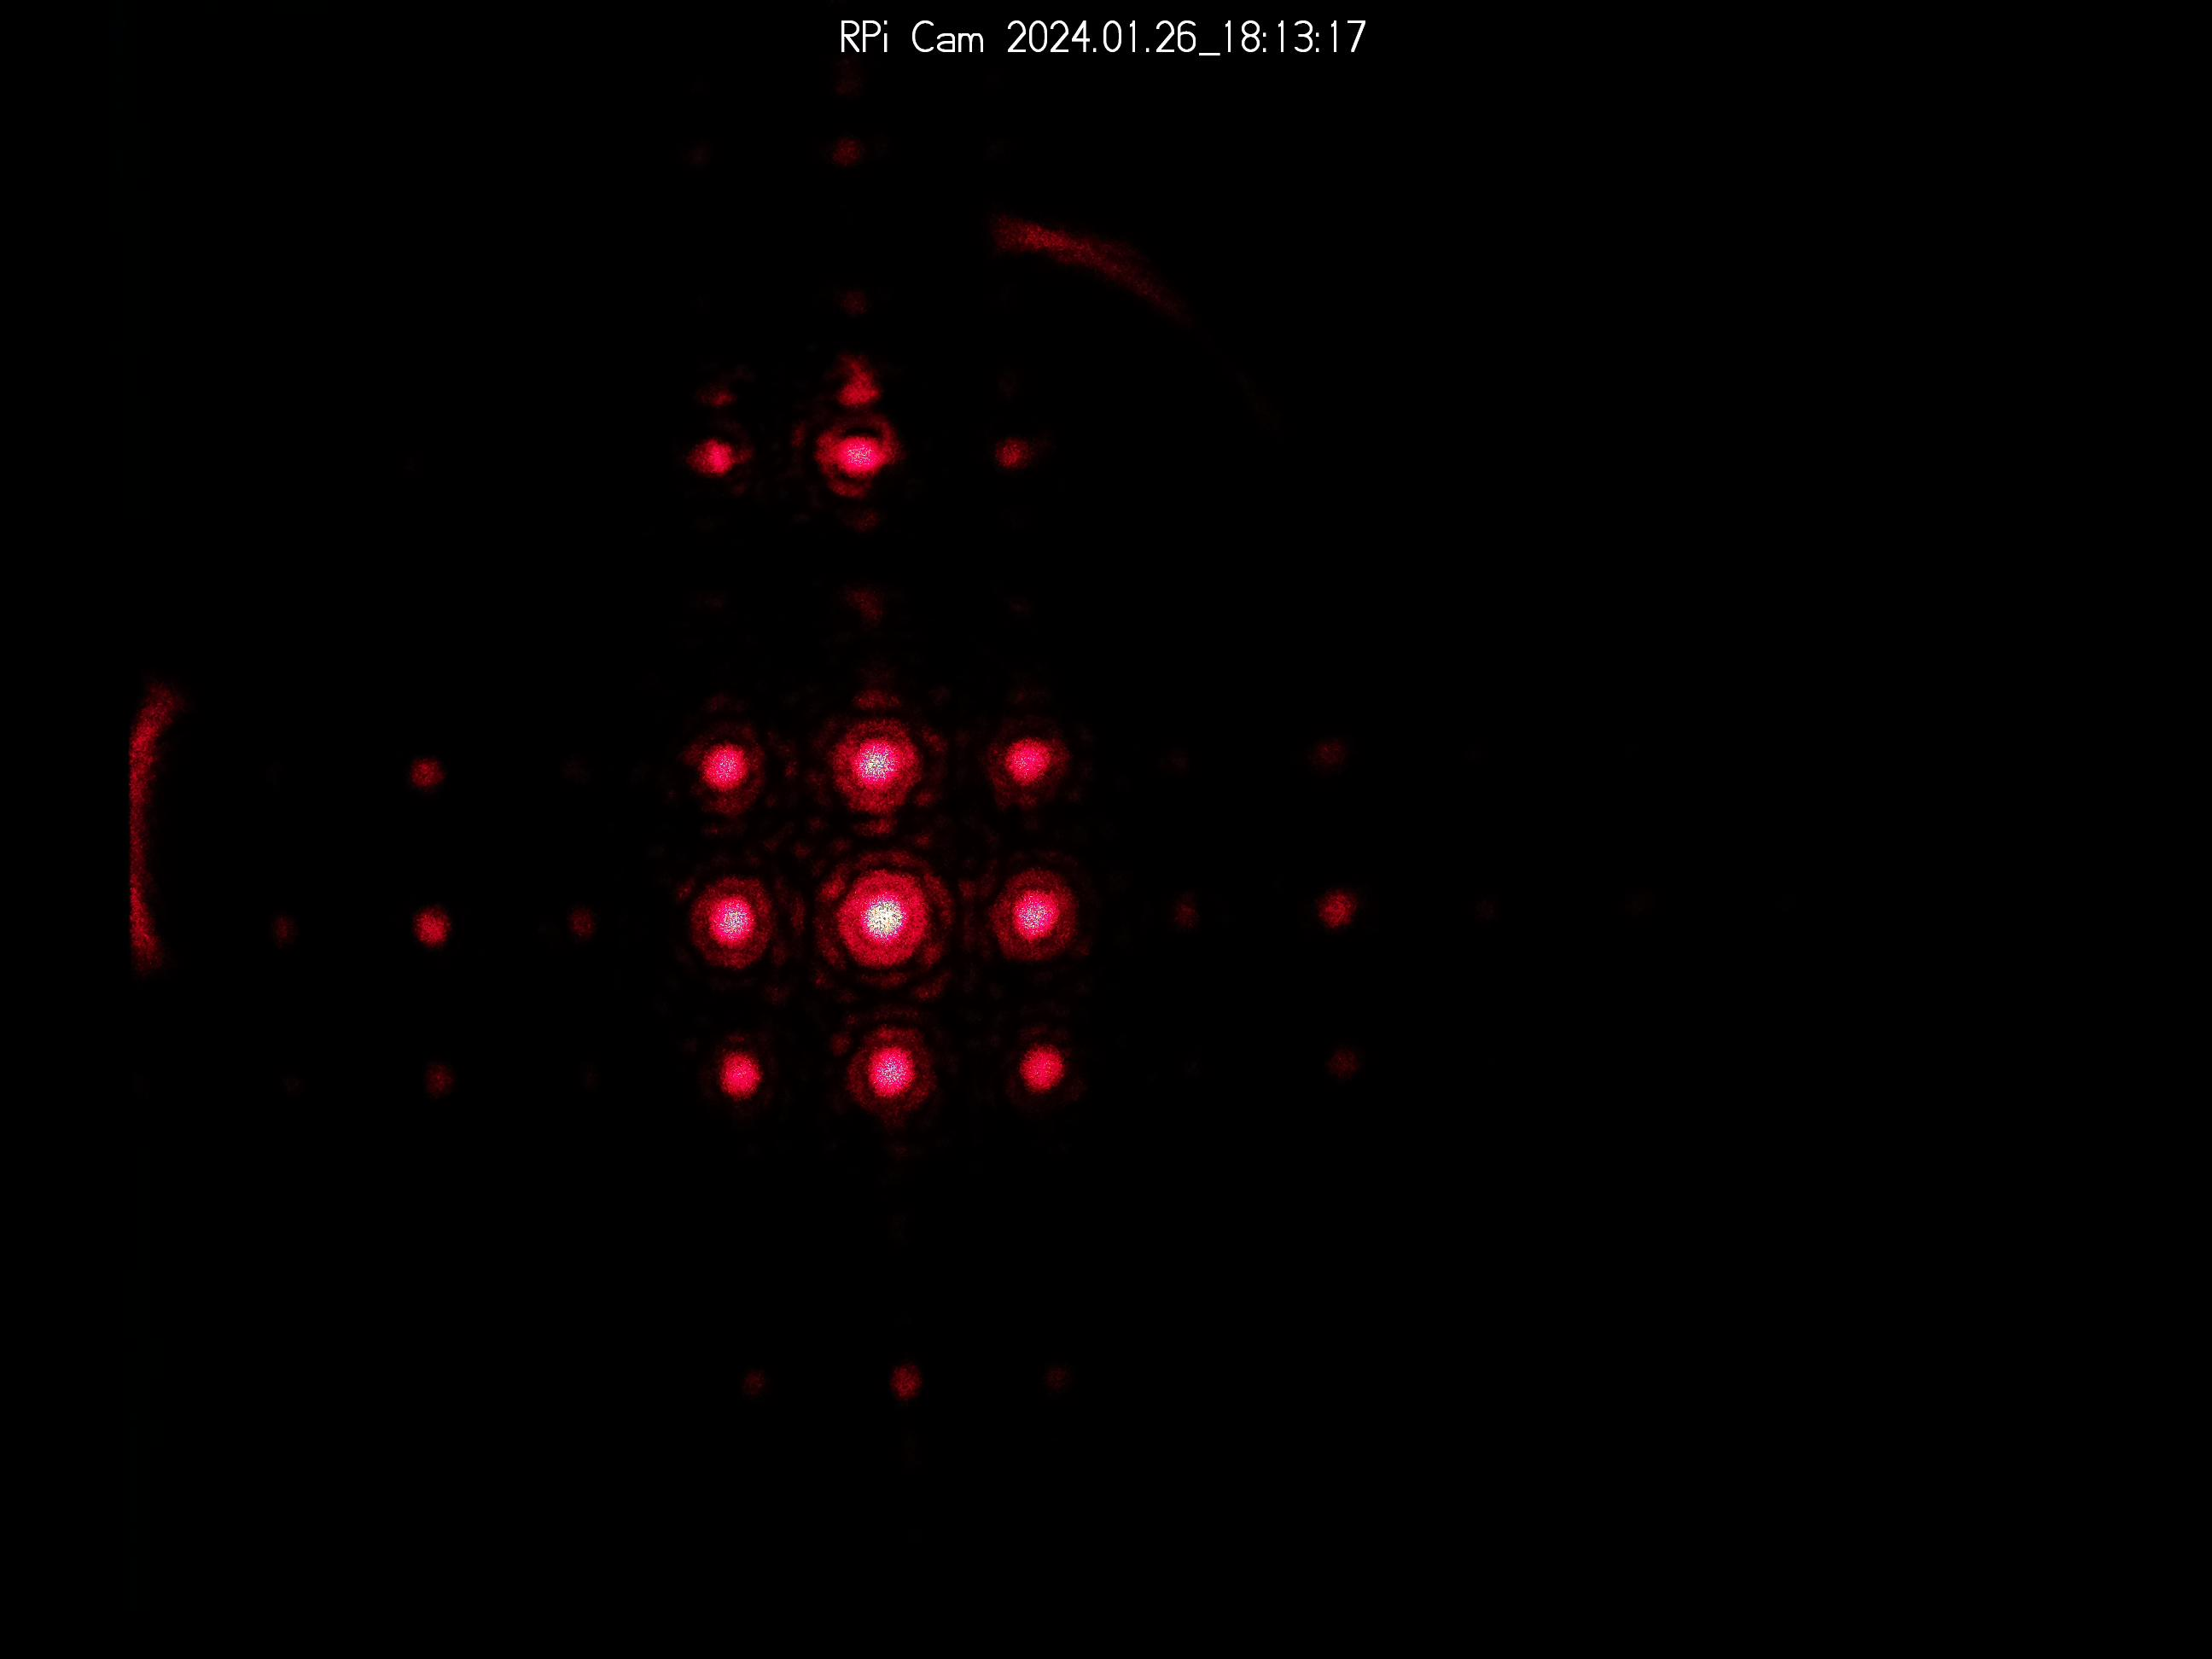
\includegraphics[width=0.5\textwidth]{Fourier/mesh_nozone/media/im_0054_20240126_181317.jpg}
    \caption{Fourier transform of the mesh for question 2.3.3C.}
    \label{fig:2-3-3C}
\end{figure}

\noindent \textcolor{red}{2.3.3D.} See figure \ref{fig:2-3-3D}. We would expect the spacial frequencies to be $k_x= \frac{x' /m}{z\lambda}$, where $m$ is the magnification ratio. Also from the original grid spacing we expect $k_x=40 cm^{-1}$. Thus $m=12.9$.

\begin{figure}[tb]
    \centering
    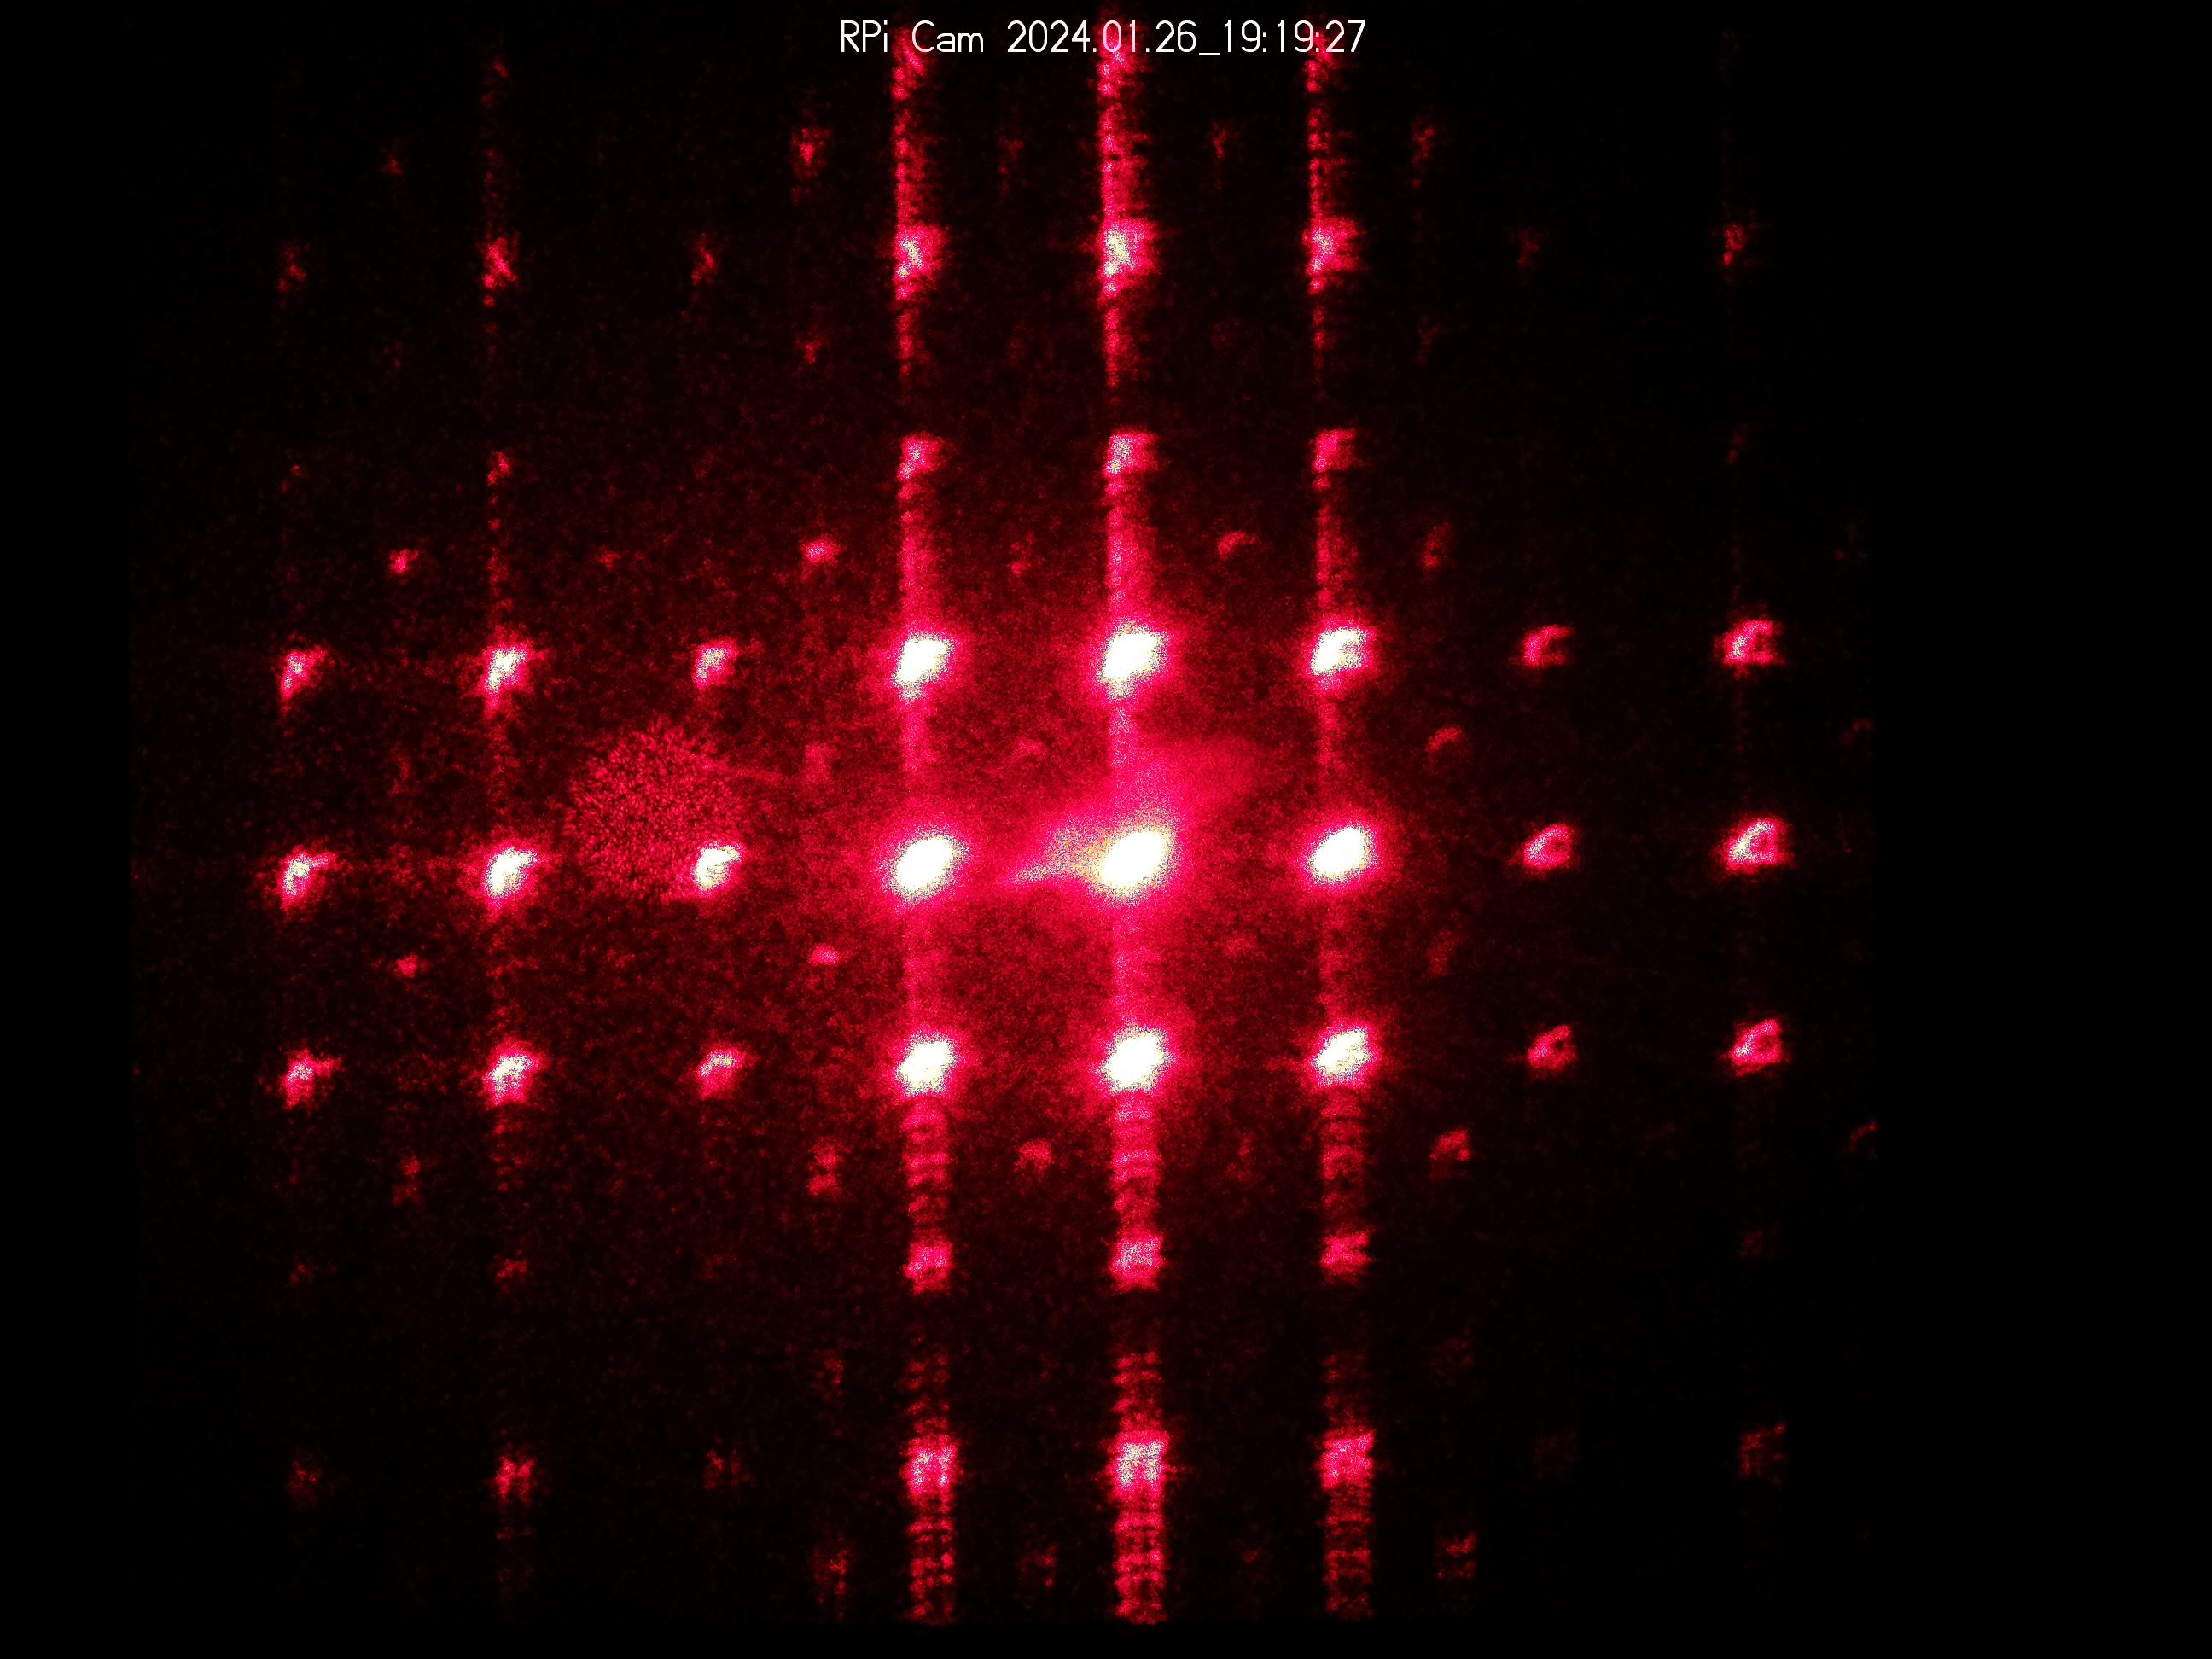
\includegraphics[width=0.5\textwidth]{Fourier/2D/media/im_0083_20240126_191927.jpg}
    \caption{Image from question 2.3.3D, this is the Fourier transform of the mesh using the FPIL.}
    \label{fig:Fourier-2D-media-im_0083_20240126_191927-jpg}
\end{figure}

\noindent \textcolor{red}{2.3.3E.} See figure \ref{fig:2-3-3E}.

\begin{figure}[tb]
    \centering
    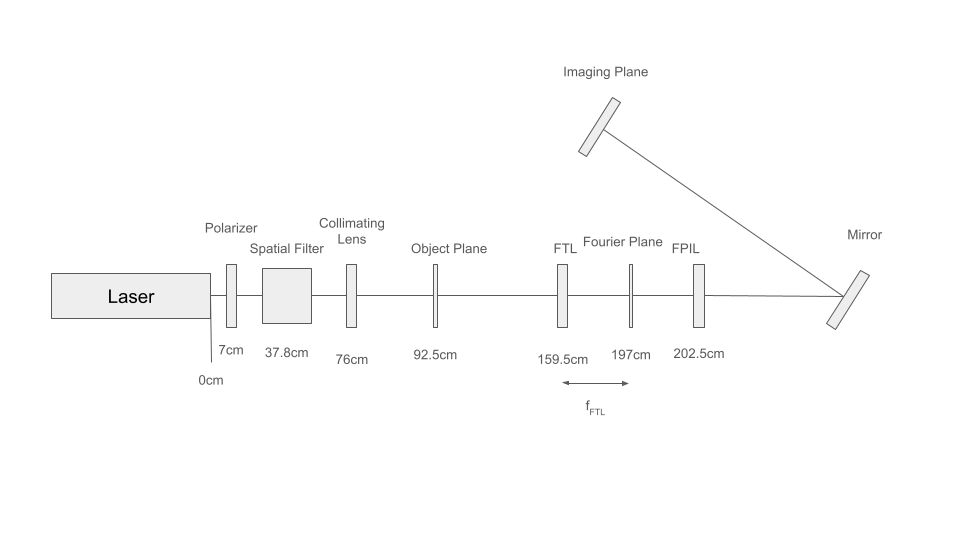
\includegraphics[width=0.8\textwidth]{2-3-3E}
    \caption{Experimental setup for 2.3.3. $f_{FTL}$ is the focus of the Fourier transform lens.}
    \label{fig:2-3-3E}
\end{figure}

\noindent \textcolor{red}{2.3.4A.} The bright spots on the Fourier transform plane represent the spatial frequencies of the mesh, which we see because of the presence of the Fourier lens after the lens.

\noindent \textcolor{red}{2.3.4B.} Translating the mesh produced no effect on the image. This is expected, since the mesh is translation invariant so the Fourier transform isn't affected. On the other hand rotating the mesh caused the dots to move closer together and get slightly less in focus. This is because after rotation the mesh is no longer in plane with the object plane, so the Fourier transform is now that of the mesh projected onto the object plane, with some focus differences coming from the lack of alignment to the object plane.

\noindent \textcolor{red}{2.3.4C.} See figure \ref{fig:2-3-4C} for the image analyzed. The distance in pixels between adjacent dots is 245 pixels, so the physical distance is $16.1$mm. From the definition of spatial frequency we have that $k_x= \frac{x'}{z\lambda}$ with $z$ in this case being the focal length for the lens, so $k_x= \frac{x' /m}{z\lambda}=3971\text{m}^{-1}$. Since the grid spacing was $40$ gaps/cm$=4000\text{m}^{-1}$, this is very close to what we'd expect.

\begin{figure}[tb]
    \centering
    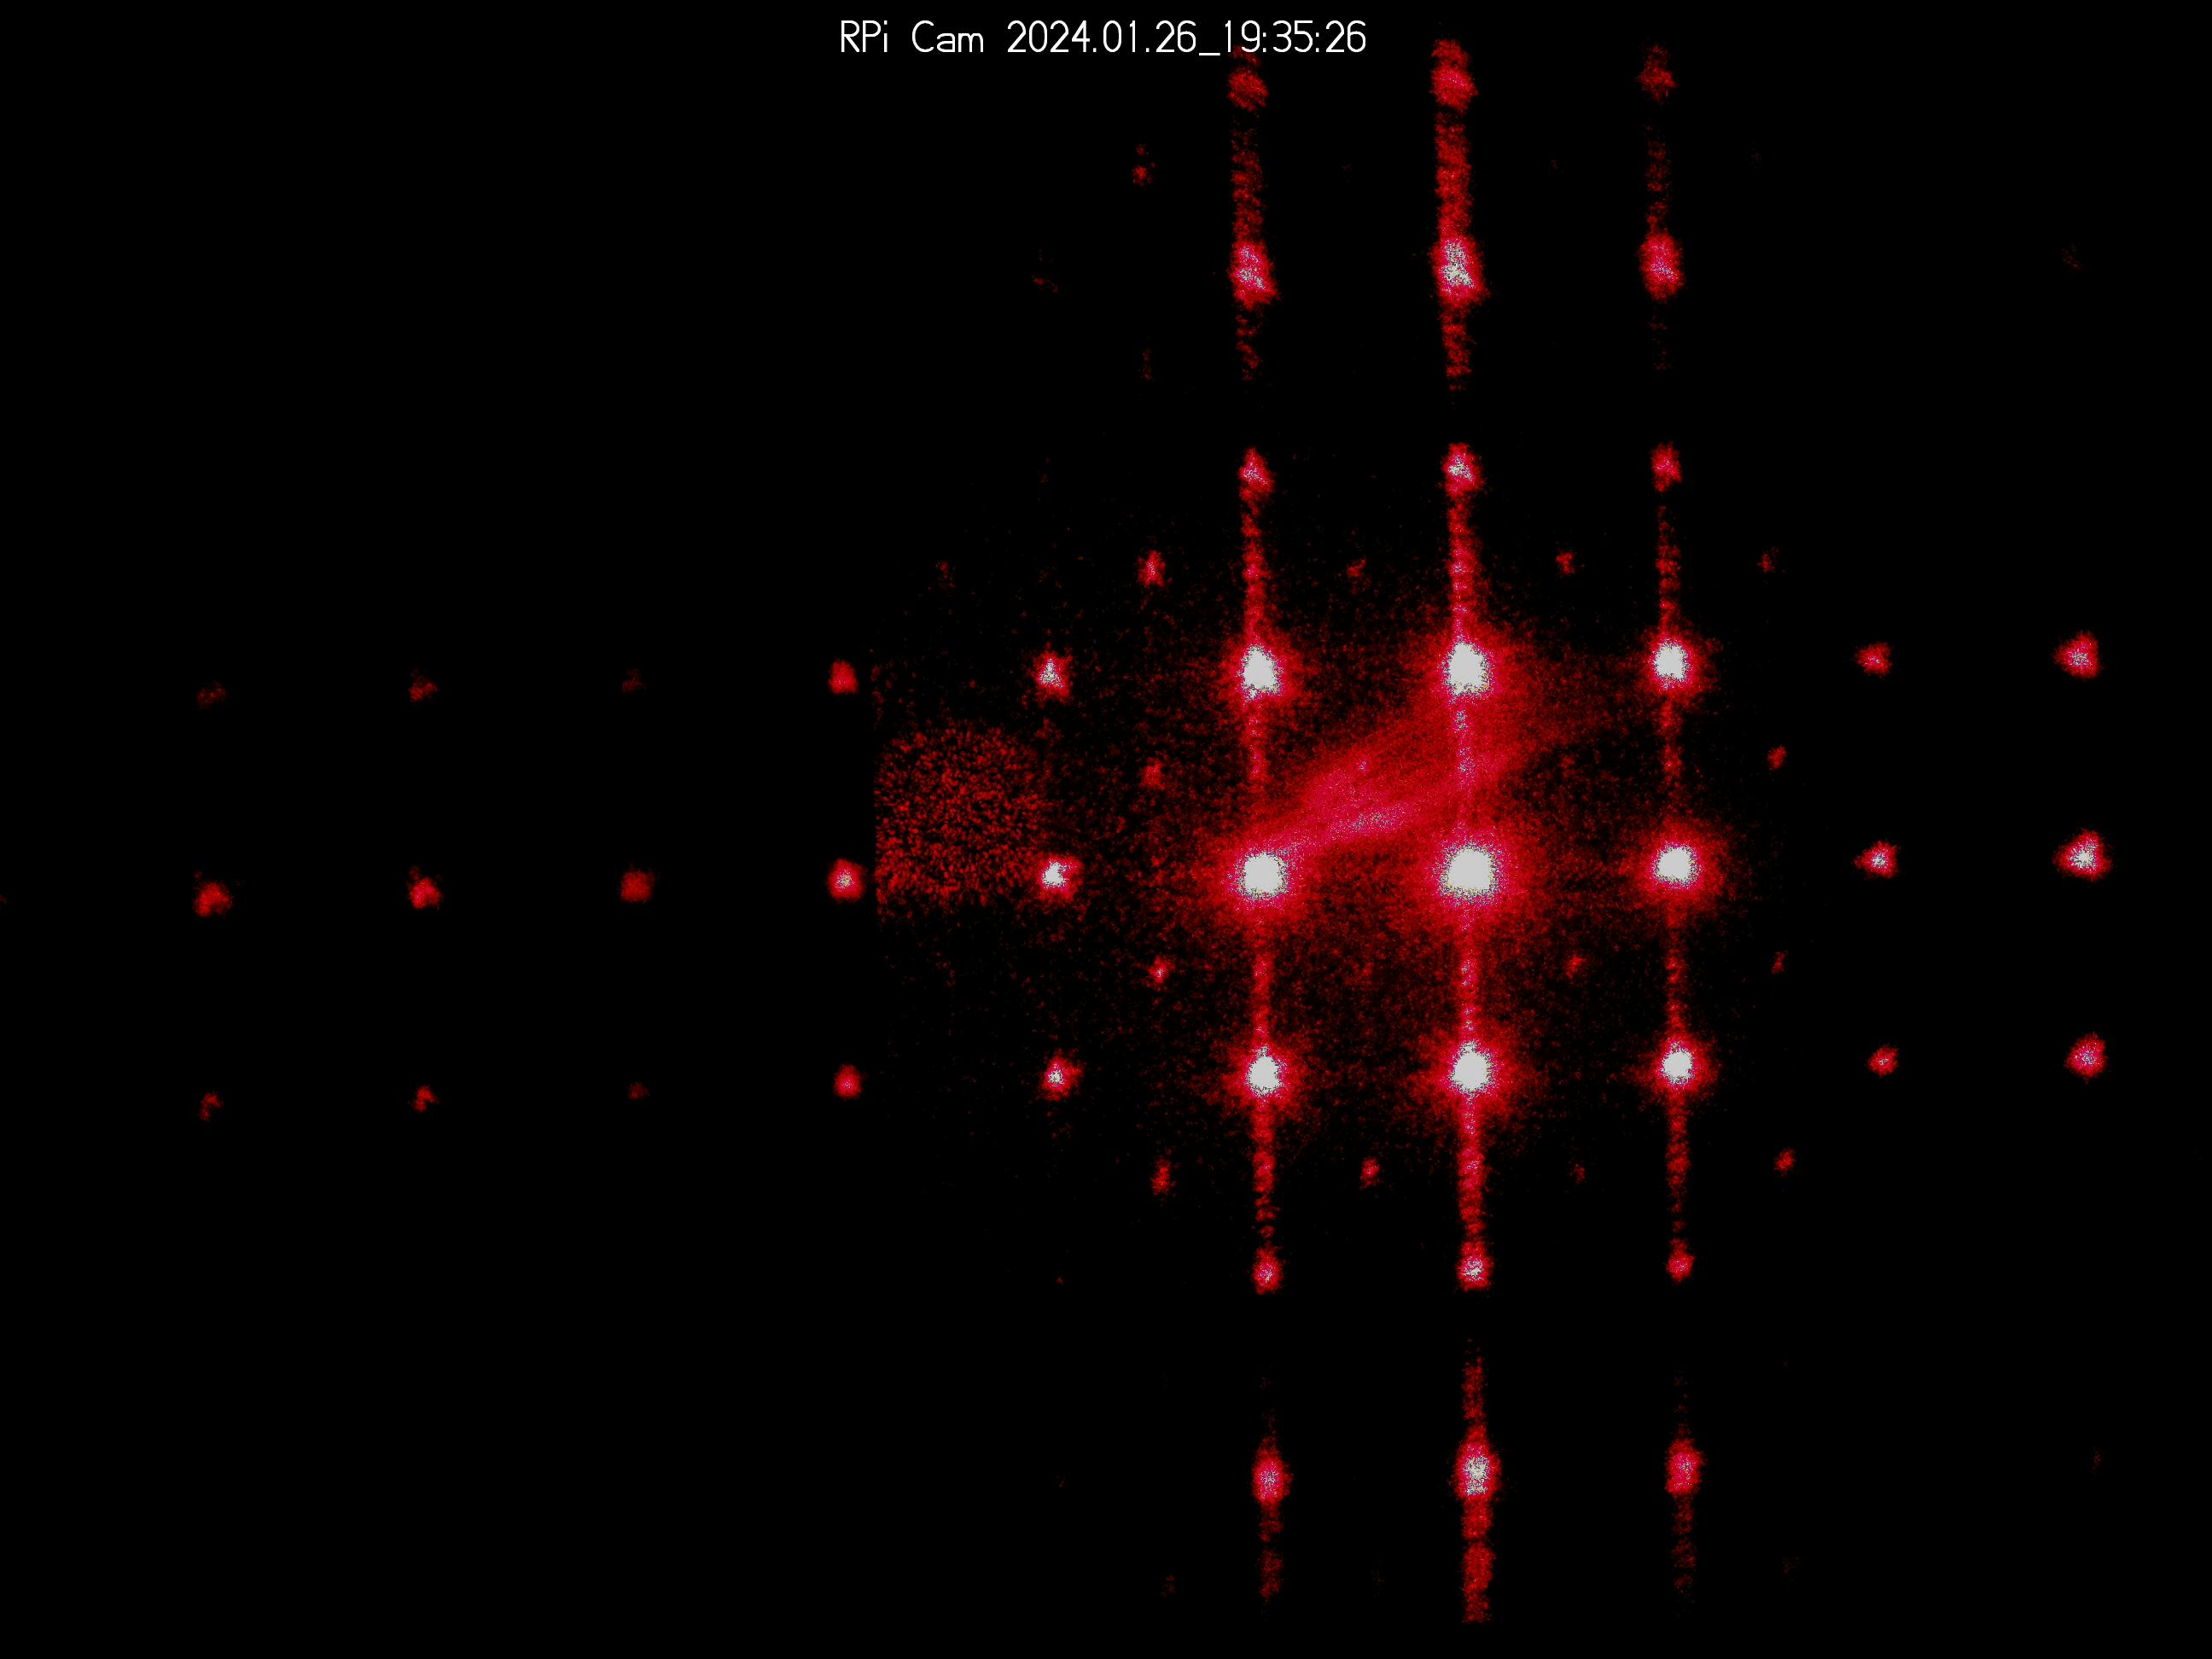
\includegraphics[width=0.5\textwidth]{Fourier/translations/media/im_0088_20240126_193526.jpg}
    \caption{Fourier transform of mesh used for 2.3.4C.}
    \label{fig:2-3-4C}
\end{figure}

\noindent \textcolor{red}{2.3.5A.} See figure \ref{fig:2-3-5A}. The procedure was to gradually shift the XY translation stage on the mount until all the dots were passed through, first centering X and then Y.

\begin{figure}[tb]
    \centering
    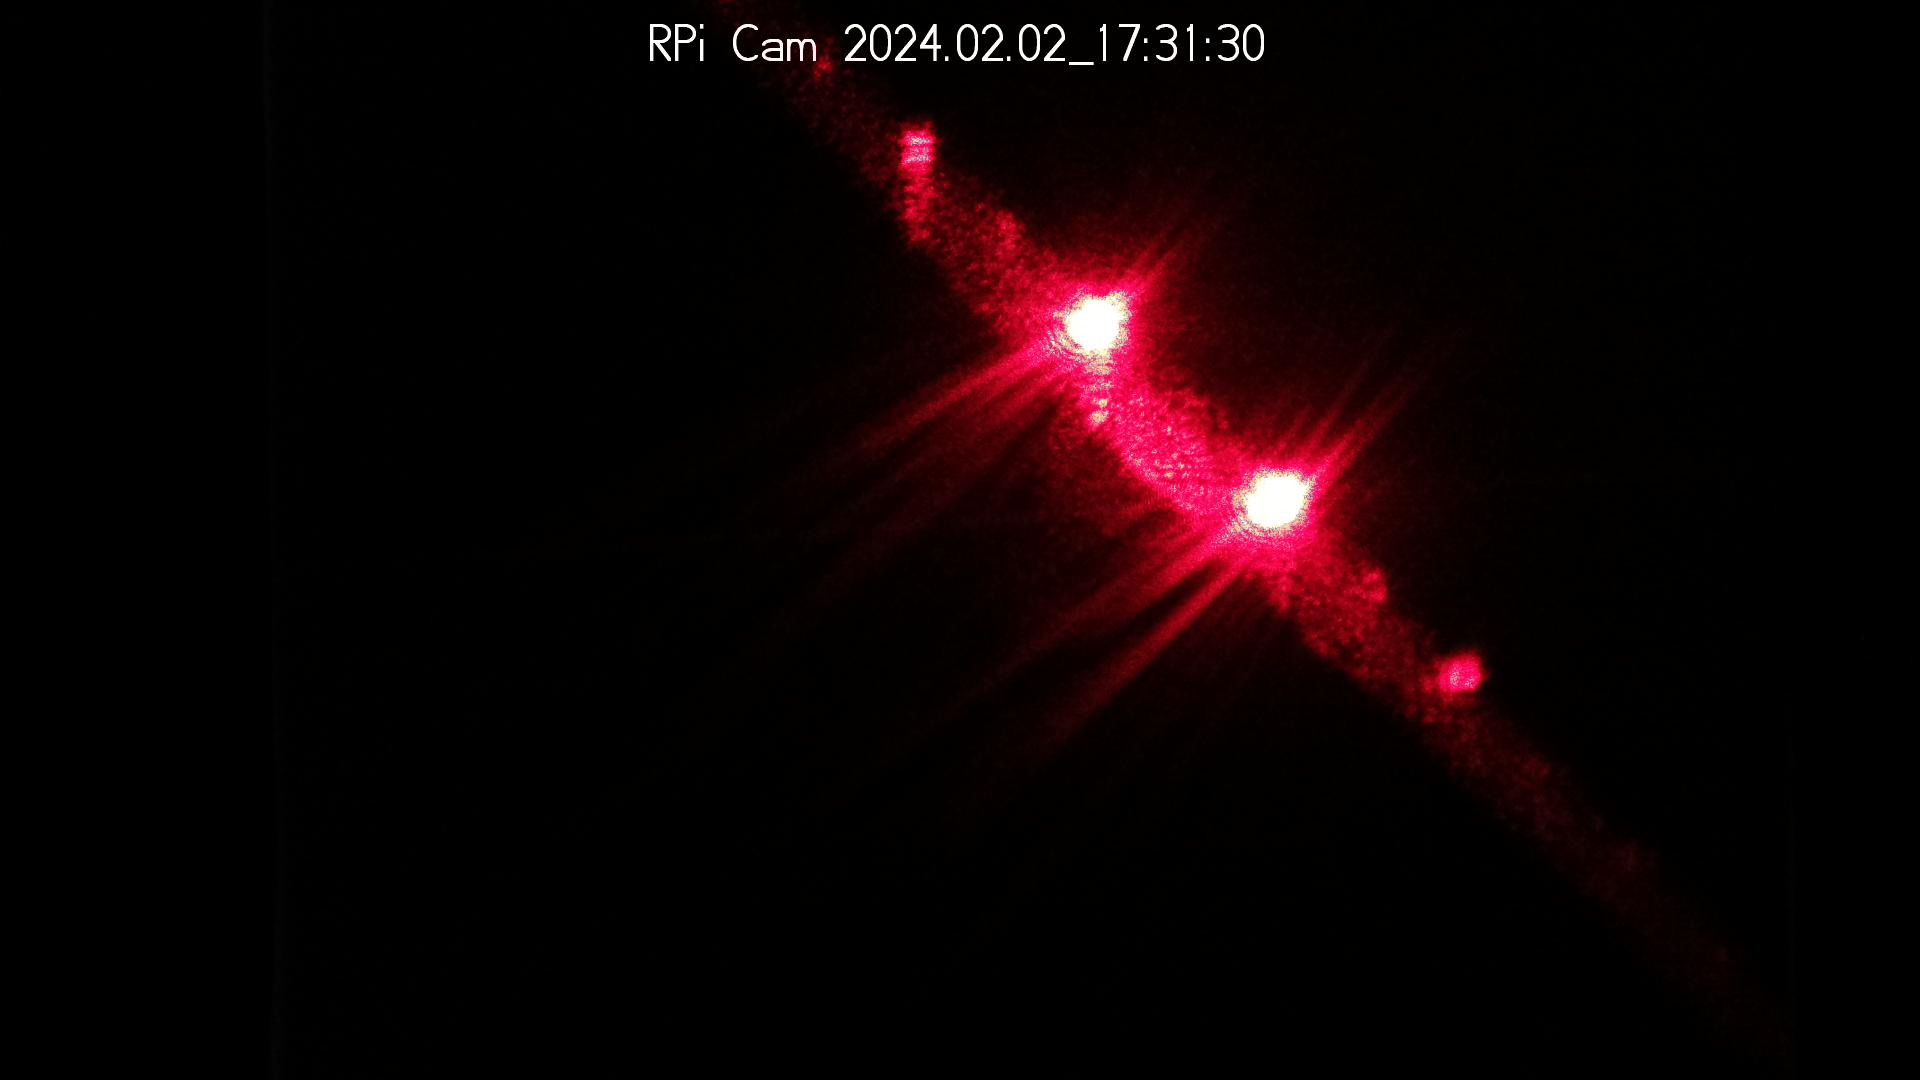
\includegraphics[width=0.45\textwidth]{Fourier/5a/media/im_0201_20240202_173130.jpg}
    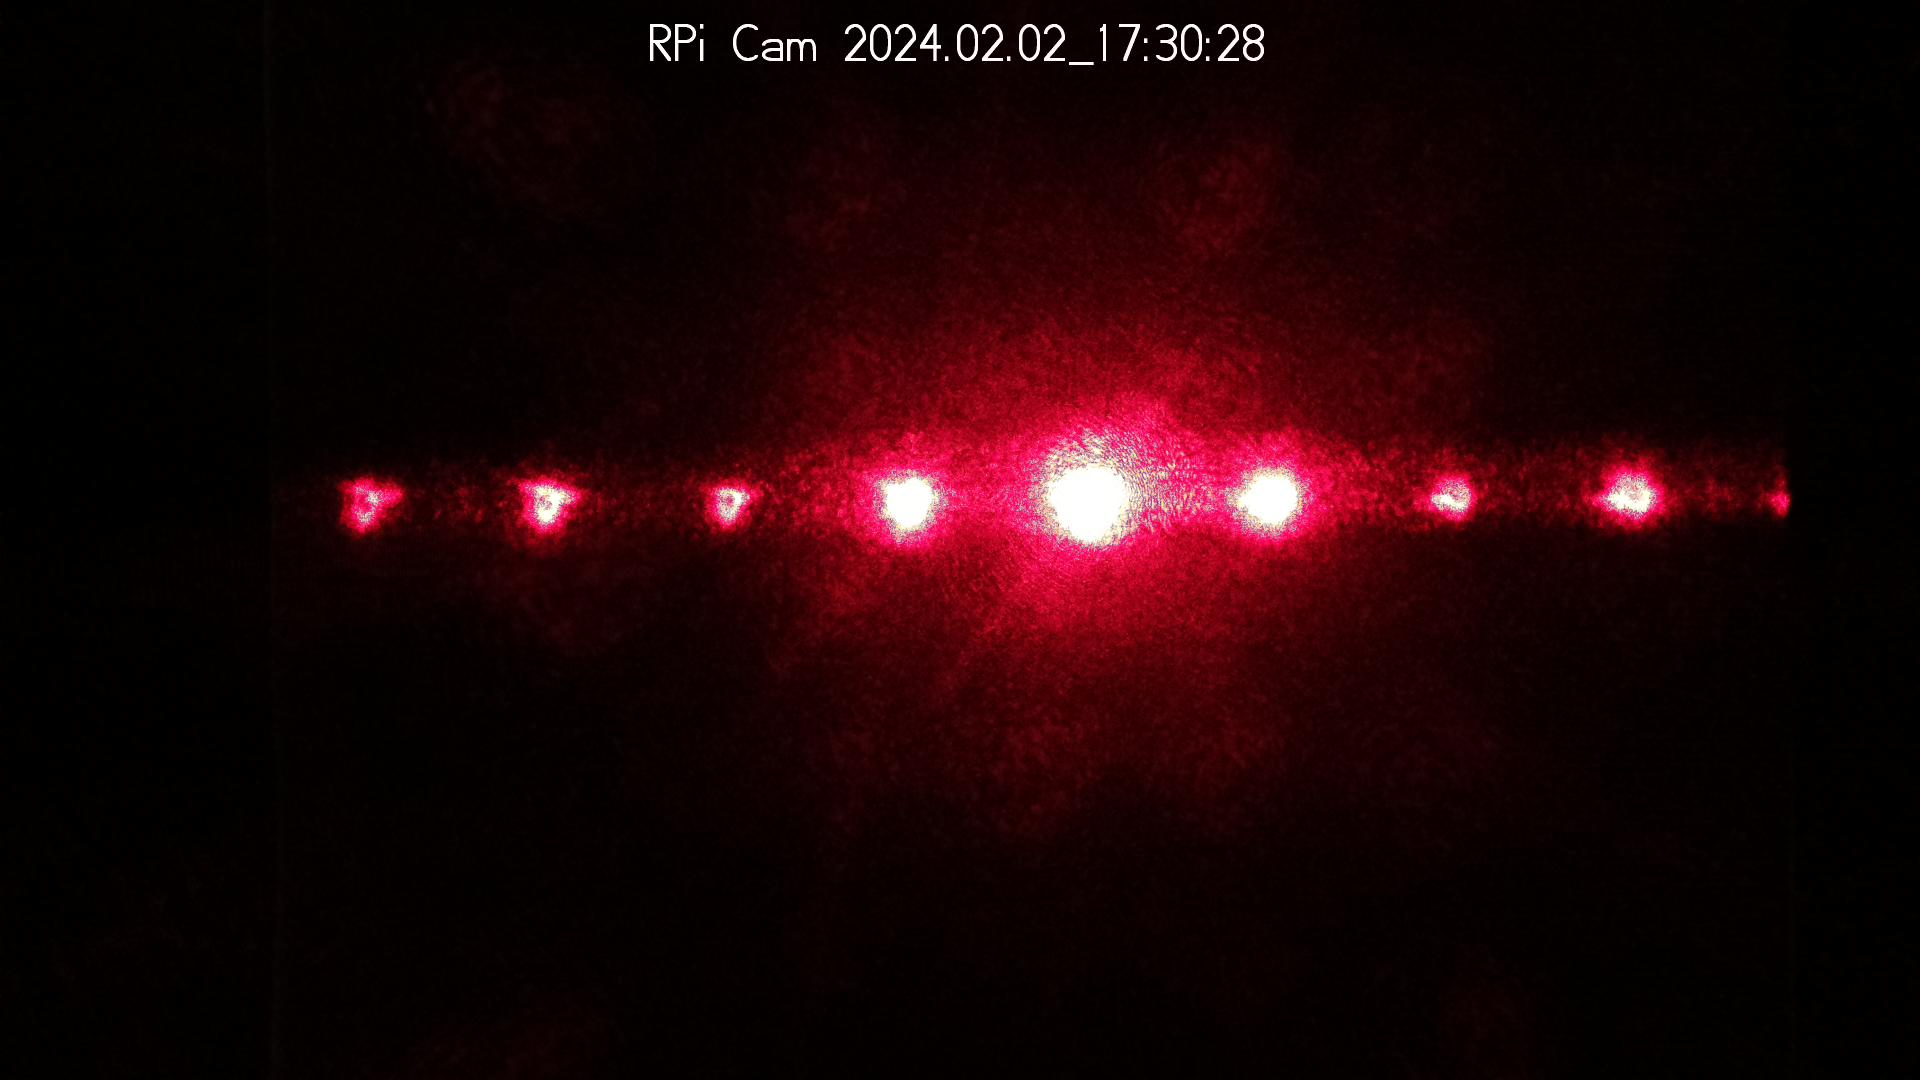
\includegraphics[width=0.45\textwidth]{Fourier/5a/media/im_0196_20240202_173028.jpg}
    \caption{Aligning the slit, on the left is rotated and the right is fully aligned.}
    \label{fig:2-3-5A}
\end{figure}

\noindent \textcolor{red}{2.3.5B.} See figure \ref{fig:2-3-5B}. This is expected. When we pass the mesh through the slit, we're effectively multiplying by a delta which removes one dimension from the Fourier transform:
\[
    \mathcal F\{t(x,y)\delta(x)\}=\int\int t(x,y)\delta(x)e^{-ik(x+y)}dxdy=\int t(0,y) e^{-iky}dy=\mathcal F\{t(0,y)\}
.\]
Thus it makes sense that passing through a vertical slit preserves only the vertical spacial frequencies.

\begin{figure}[tb]
    \centering
    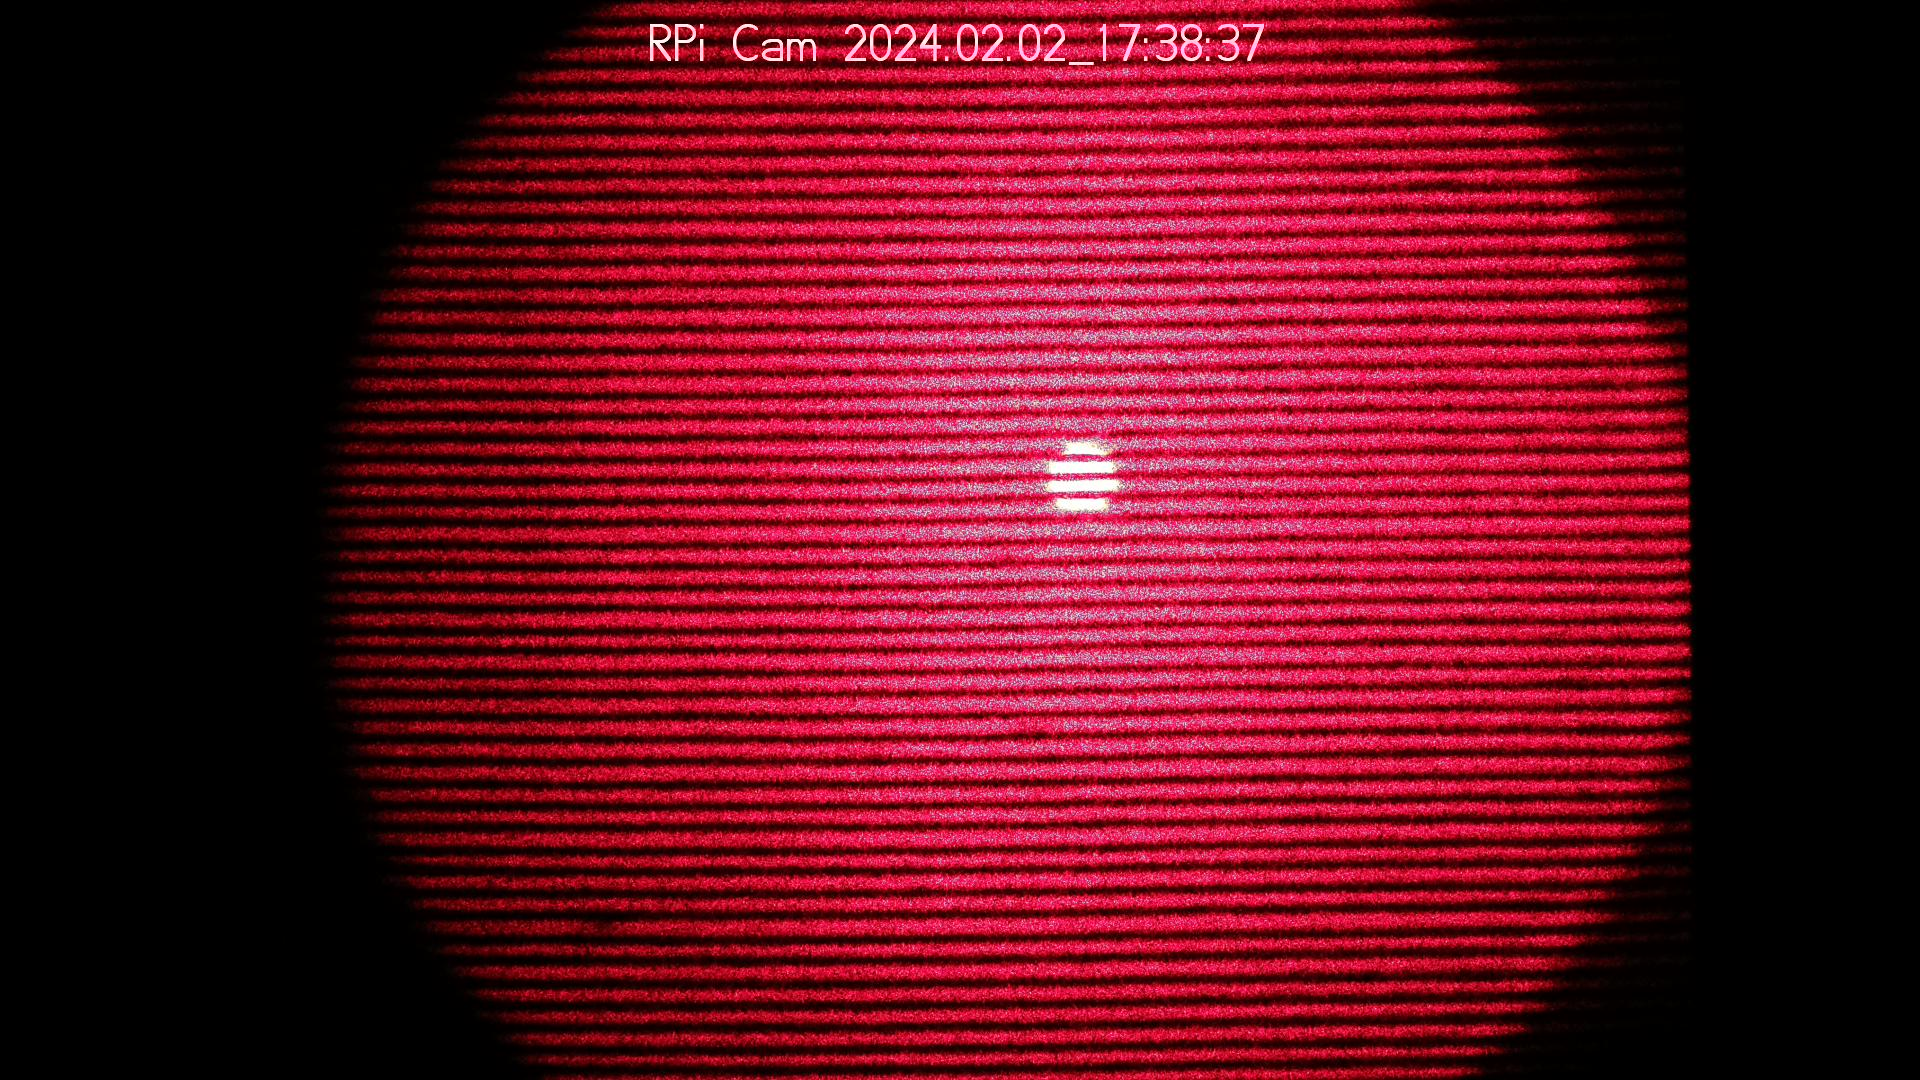
\includegraphics[width=0.8\textwidth]{Fourier/5b/media/im_0203_20240202_173838.jpg}
    \caption{Image of mesh passing through slit after removing FPIL. The horizontal bars come from removing one dimension of the fourier transform, see 2.3.5B for the explanation.}
    \label{fig:2-3-5B}
\end{figure}

\noindent \textcolor{red}{2.3.5C.} The spatial filter is effectively exactly what we're doing here, except instead of a slit it uses a pinhole. By using a lens to focus the beam and placing a pinhole at the focus plane, all frequencies except the low, uniform frequency is filtered out. Thus any noise present after the HeNe laser is completely filtered out, and only the low spatial frequencies representing uniform light remains.

\noindent \textcolor{red}{2.3.5D.} See figure \ref{fig:2-3-5D}. The diagonal $45^{\circ}$ lines are because we're effectively taking the Fourier transform of the same thing. Recall figure \ref{fig:2-3-5A}, after the slit it's effectively a combination of many intense dots. When we rotate the slit the function we're taking the Fourier transform is the exact same, just scaled by a factor of approximately $\frac{1}{\sqrt{2}}$ because the geometry of the square we're bisecting with the slit now.

\begin{figure}[tb]
    \centering
    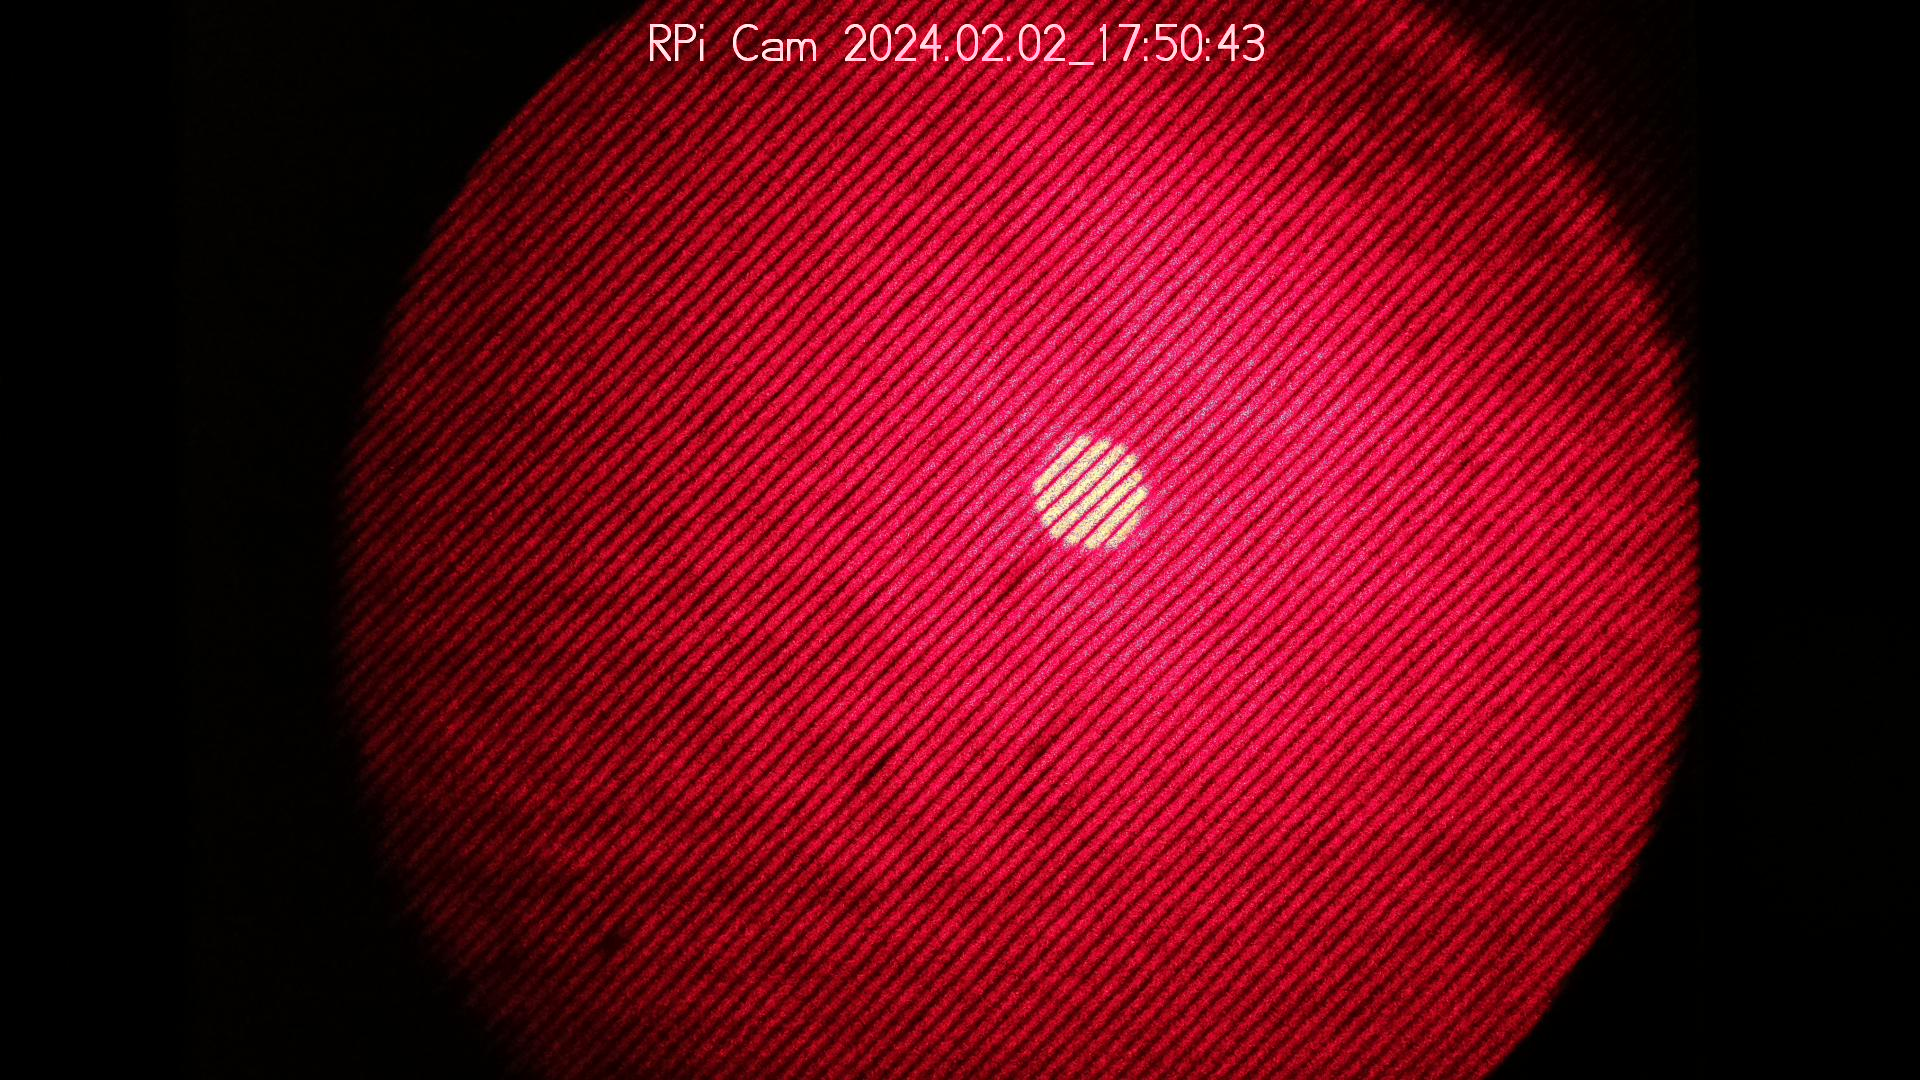
\includegraphics[width=0.8\textwidth]{Fourier/5d/media/im_0208_20240202_175043.jpg}
    \caption{Diagonal lines resulting from rotating the slit.}
    \label{fig:2-3-5D}
\end{figure}

\noindent \textcolor{red}{2.3.5E.} See figure \ref{fig:2-3-5E}. The reason the FT of the NOZONE is more complex is simply because it's fundamentally a more complicated shape. Unlike a mesh which can be represented cleanly by a sum of delta functions, human readable text is rather arbitrary so there's no reason we'd expect it to be some kind of simple pattern.

\begin{figure}[tb]
    \centering
    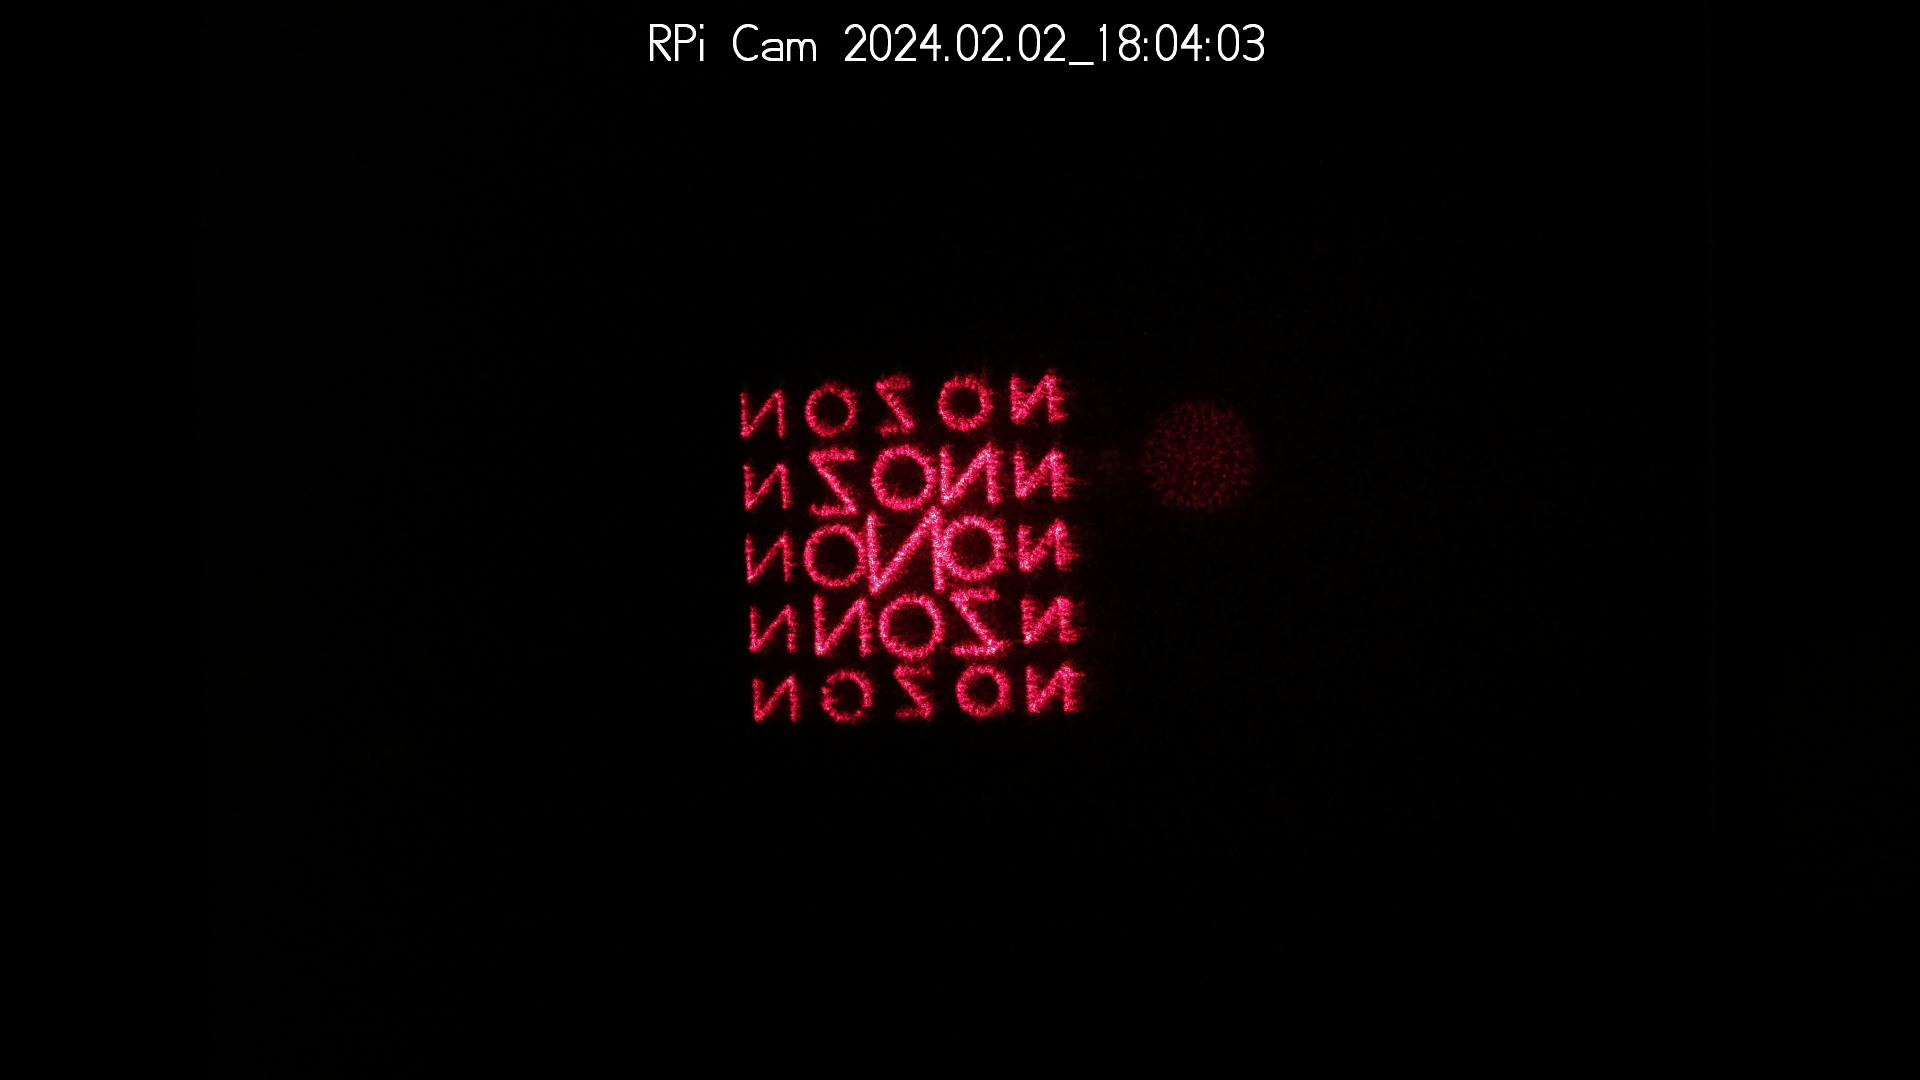
\includegraphics[width=0.45\textwidth]{Fourier/5e/media/im_0211_20240202_180403.jpg}
    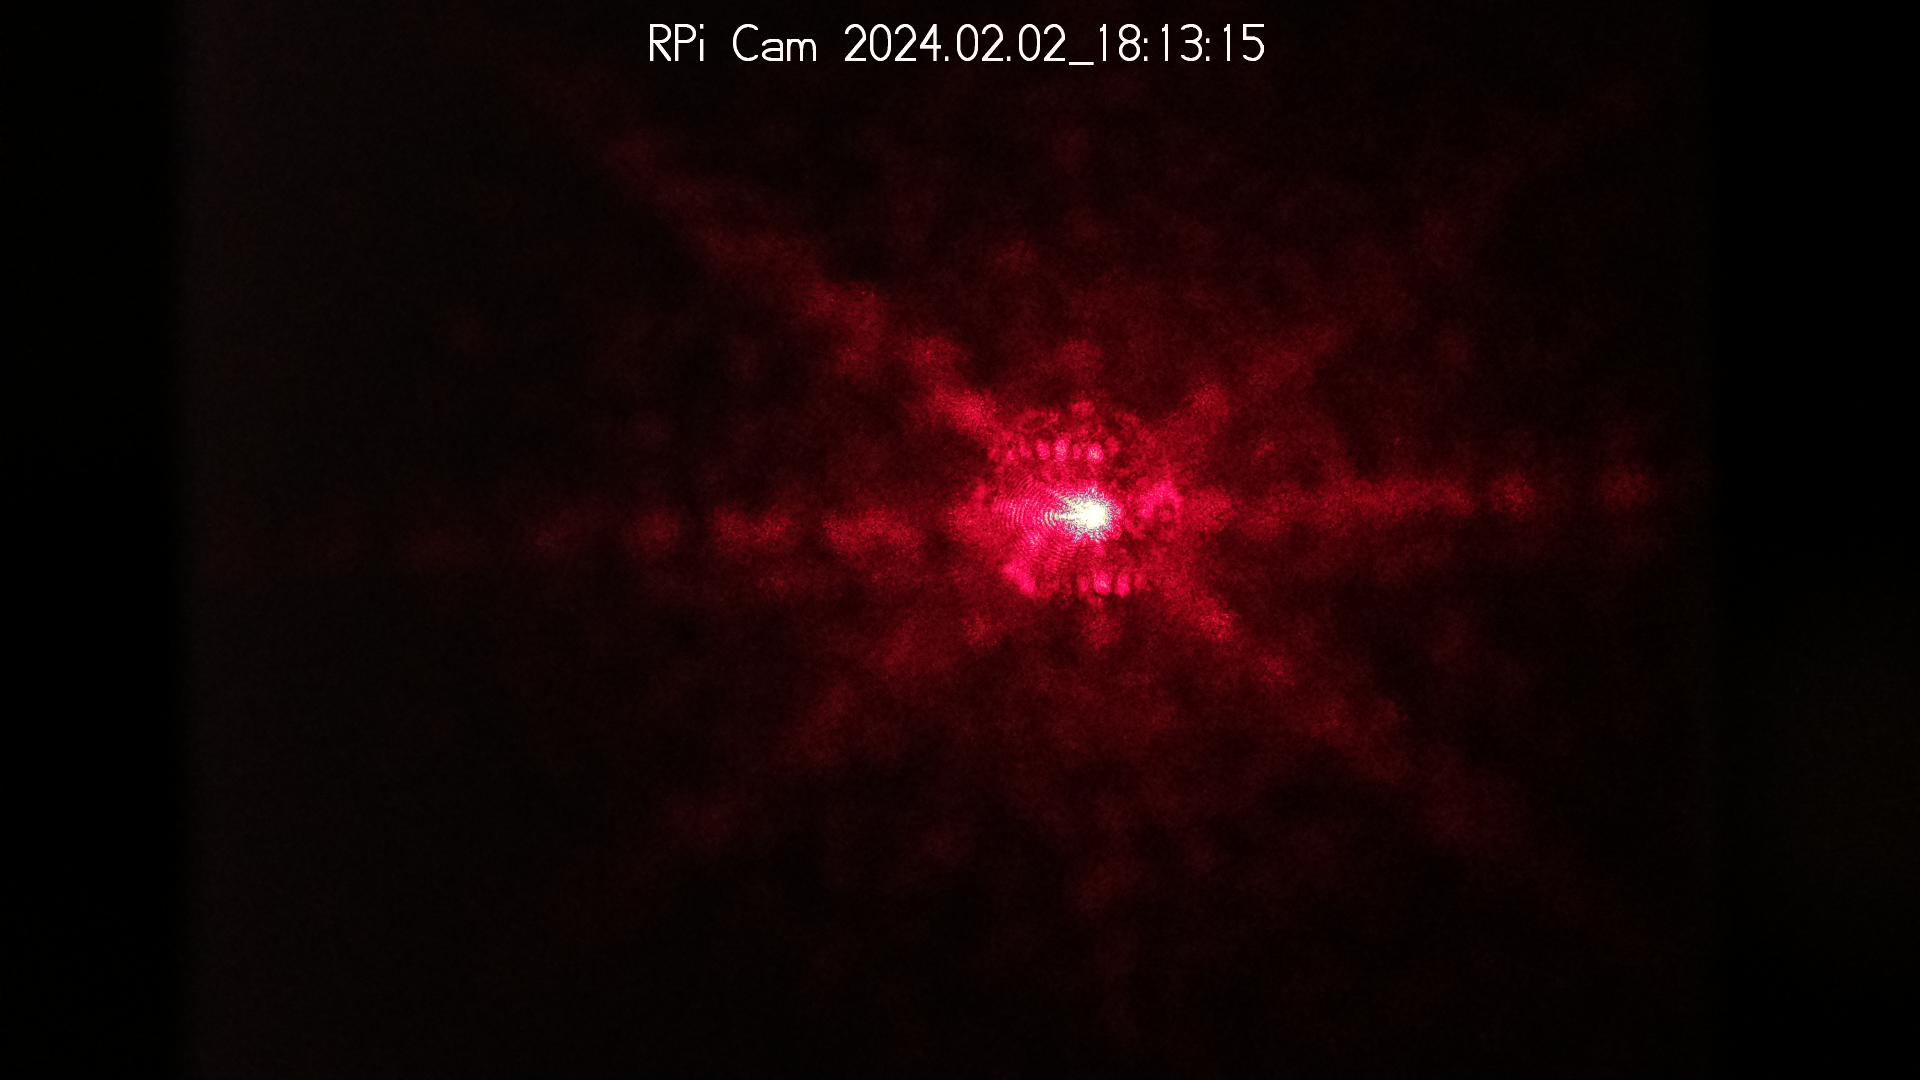
\includegraphics[width=0.45\textwidth]{Fourier/5e/media/im_0216_20240202_181315.jpg}
    \caption{Direct image of NOZONE (left) and its Fourier transform (right)}
    \label{fig:2-3-5E}
\end{figure}

\noindent \textcolor{red}{2.3.5F.} The approach that worked well was to use the X filter oriented with the one axis aligned vertically and the other aligned in the same direction as the N's diagonal line. See figure \ref{fig:2-3-5F} for the resulting filtered image. It's not completely perfect, but the Ns are clearly much more visible and other letters are quite faded.

\begin{figure}[tb]
    \centering
    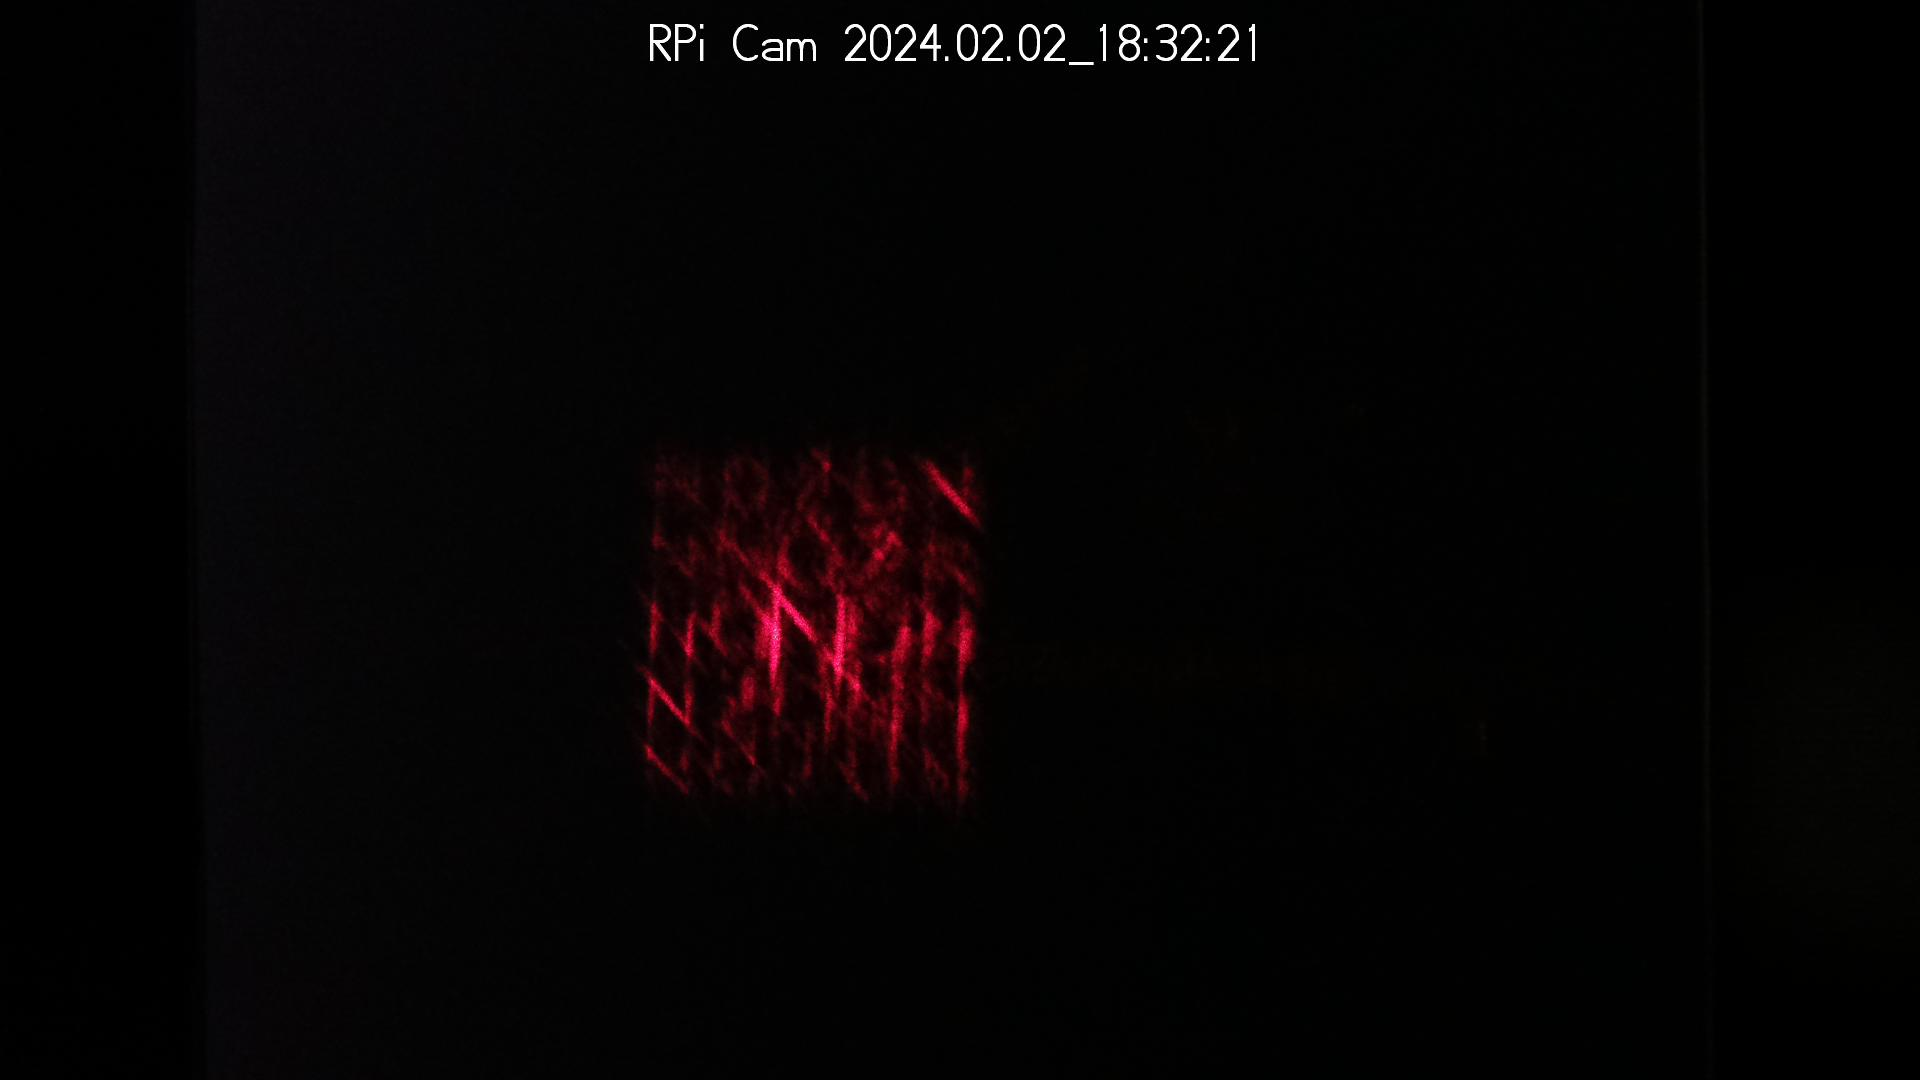
\includegraphics[width=0.8\textwidth]{Fourier/5f/media/im_0219_20240202_183221.jpg}
    \caption{Filtered NOZONE image for just the Ns.}
    \label{fig:2-3-5F}
\end{figure}

\noindent \textcolor{red}{2.3.5G.} See figure \ref{fig:2-3-5G}. Since the dot filters out the low spatial frequency of the light, only the higher frequency components remain. In practice, this has the effect of attenuating any edges and fine detail significantly, since these are the parts of the image that require high frequency components to accurately represent.

\begin{figure}[tb]
    \centering
    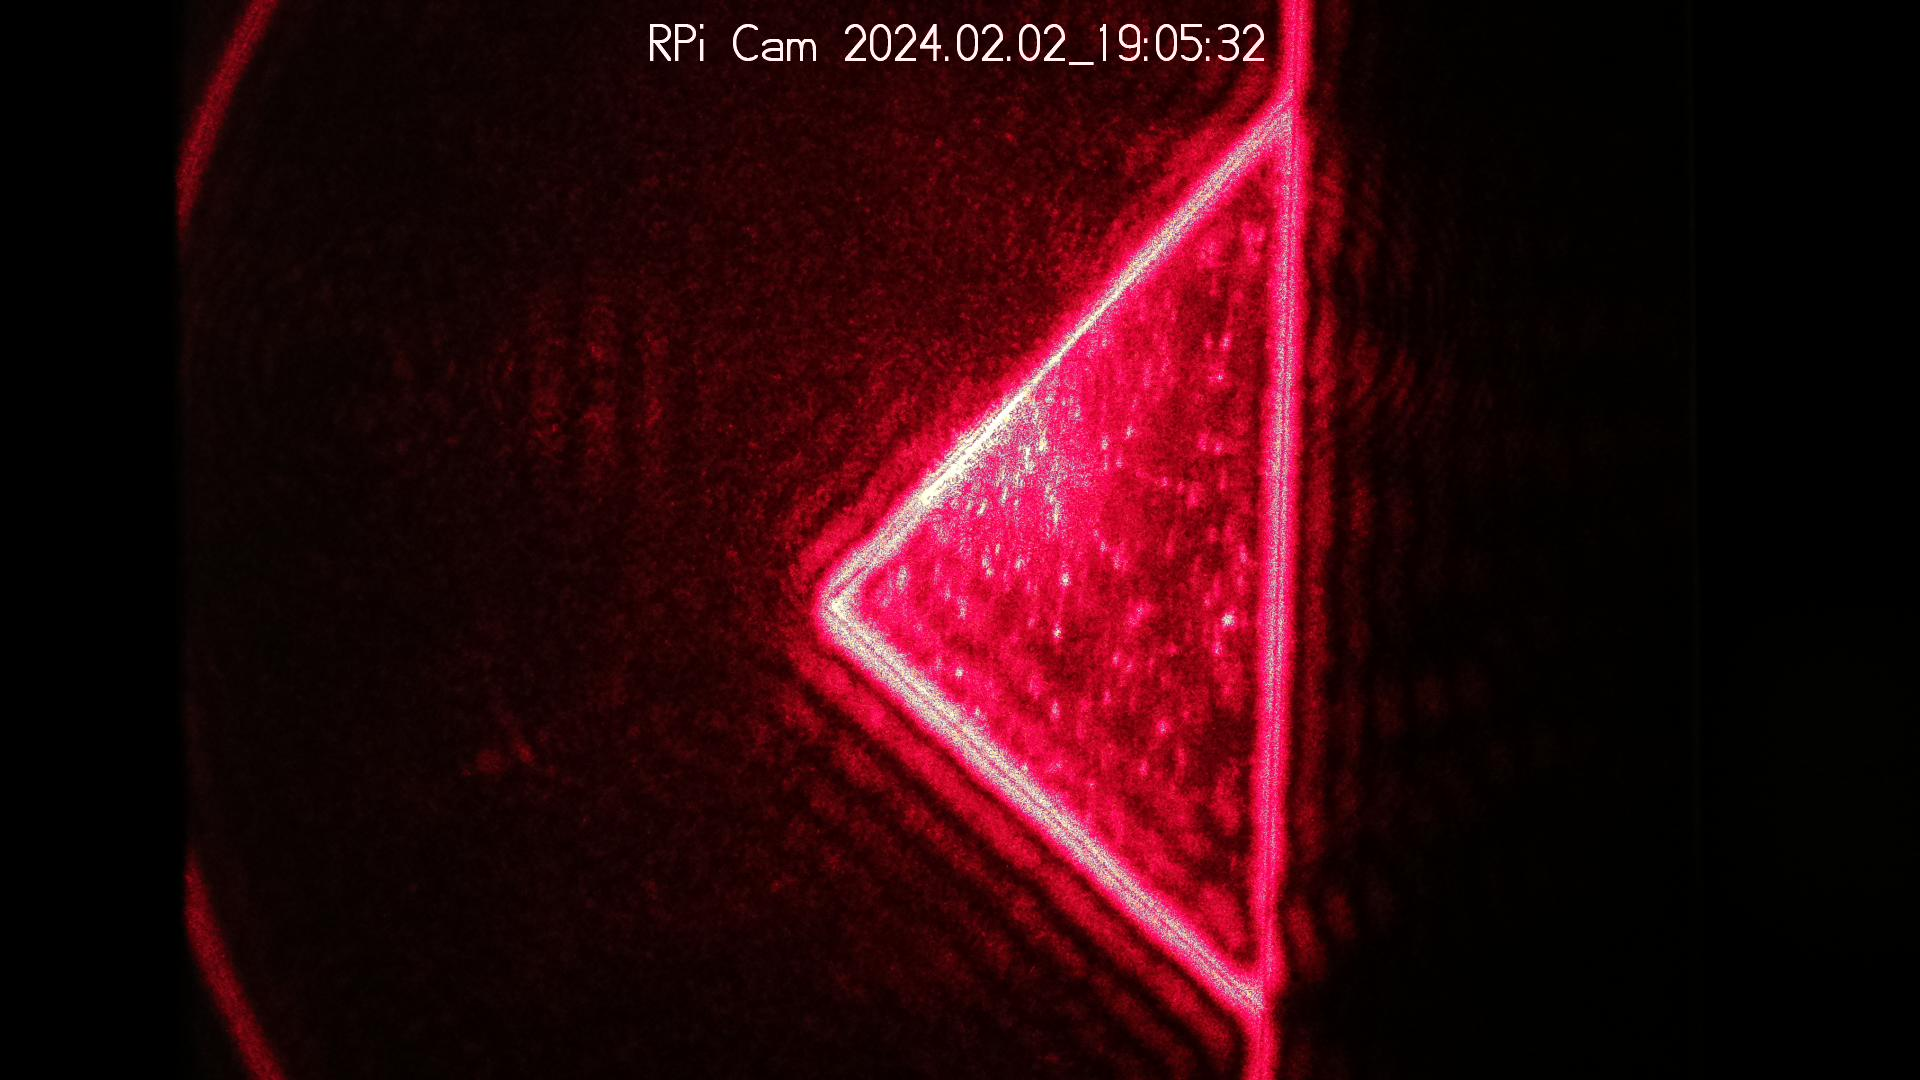
\includegraphics[width=0.8\textwidth]{Fourier/5g/media/im_0229_20240202_190532.jpg}
    \caption{The razorblade after being filtered for low frequency light. Note how the edges are extremely attenuated.}
    \label{fig:2-3-5G}
\end{figure}

\end{document}
